\documentclass[11pt,a4paper]{article}
\usepackage[T1]{fontenc}
\usepackage[utf8]{inputenc}
\usepackage{lmodern}
\usepackage[margin=2.5cm]{geometry}
\usepackage{amsmath}
\usepackage{graphicx}
\usepackage{booktabs}
\usepackage{array}
\usepackage[section]{placeins}
\usepackage{caption}
\usepackage{enumitem}
\usepackage[hidelinks]{hyperref}
\usepackage{xurl}
\captionsetup{font=small,labelfont=bf}
\setlist{itemsep=2pt,topsep=4pt}
\expandafter\def\csname res@Tc\endcsname{3272}
\expandafter\def\csname res@altApForty\endcsname{227}
\expandafter\def\csname res@altApTwenty\endcsname{190}
\expandafter\def\csname res@altGainHigh\endcsname{1.3}
\expandafter\def\csname res@altGainLow\endcsname{2.4}
\expandafter\def\csname res@altVForty\endcsname{240\,000}
\expandafter\def\csname res@altVTwenty\endcsname{4\,500}
\expandafter\def\csname res@altVolRatioHigh\endcsname{8.9}
\expandafter\def\csname res@altVolRatioLow\endcsname{6.0}
\expandafter\def\csname res@atmP\endcsname{1197}
\expandafter\def\csname res@atmRho\endcsname{0.0184}
\expandafter\def\csname res@atmT\endcsname{226.5}
\expandafter\def\csname res@audDiv\endcsname{60.45}
\expandafter\def\csname res@audDvBack\endcsname{2173}
\expandafter\def\csname res@audDvPct\endcsname{24}
\expandafter\def\csname res@audEratio\endcsname{34}
\expandafter\def\csname res@audGasRatio\endcsname{11.5}
\expandafter\def\csname res@audH2ratio\endcsname{70}
\expandafter\def\csname res@audLnA\endcsname{0.916}
\expandafter\def\csname res@audLnB\endcsname{1.253}
\expandafter\def\csname res@audMolar\endcsname{947}
\expandafter\def\csname res@audPratio\endcsname{9.8}
\expandafter\def\csname res@audRhoLow\endcsname{1.8}
\expandafter\def\csname res@audRhoRatio\endcsname{10.4}
\expandafter\def\csname res@audRhoTot\endcsname{56}
\expandafter\def\csname res@audVolRatio\endcsname{6.1}
\expandafter\def\csname res@balAp\endcsname{214}
\expandafter\def\csname res@balArea\endcsname{4347}
\expandafter\def\csname res@balBareH2\endcsname{22.5}
\expandafter\def\csname res@balBareV\endcsname{17\,600}
\expandafter\def\csname res@balDv\endcsname{2091}
\expandafter\def\csname res@balEnv\endcsname{130}
\expandafter\def\csname res@balEps\endcsname{36.4}
\expandafter\def\csname res@balF\endcsname{11.8}
\expandafter\def\csname res@balH2\endcsname{34.5}
\expandafter\def\csname res@balHb\endcsname{58.0}
\expandafter\def\csname res@balHe\endcsname{75.4}
\expandafter\def\csname res@balHeMassRatio\endcsname{2.18}
\expandafter\def\csname res@balHeVolPct\endcsname{10}
\expandafter\def\csname res@balIsp\endcsname{303.4}
\expandafter\def\csname res@balIspVac\endcsname{307.3}
\expandafter\def\csname res@balLaunchH2\endcsname{38}
\expandafter\def\csname res@balLd\endcsname{8}
\expandafter\def\csname res@balLg\endcsname{369}
\expandafter\def\csname res@balMdot\endcsname{3.97}
\expandafter\def\csname res@balPe\endcsname{4.7}
\expandafter\def\csname res@balQ\endcsname{1.7}
\expandafter\def\csname res@balTap\endcsname{222}
\expandafter\def\csname res@balTb\endcsname{38.1}
\expandafter\def\csname res@balV\endcsname{27\,000}
\expandafter\def\csname res@balVHe\endcsname{29\,600}
\expandafter\def\csname res@balVHi\endcsname{30\,300}
\expandafter\def\csname res@balVLo\endcsname{24\,000}
\expandafter\def\csname res@balVb\endcsname{1714}
\expandafter\def\csname res@betaBase\endcsname{2397}
\expandafter\def\csname res@betaHi\endcsname{4506}
\expandafter\def\csname res@betaLo\endcsname{1046}
\expandafter\def\csname res@bmCstar\endcsname{1726}
\expandafter\def\csname res@bmFrozen\endcsname{274.9}
\expandafter\def\csname res@bmShift\endcsname{285.9}
\expandafter\def\csname res@bmTc\endcsname{3426}
\expandafter\def\csname res@cBalD\endcsname{0.31}
\expandafter\def\csname res@cBalDry\endcsname{90.4}
\expandafter\def\csname res@cBalEnv\endcsname{89}
\expandafter\def\csname res@cBalF\endcsname{5.5}
\expandafter\def\csname res@cBalGas\endcsname{19.3}
\expandafter\def\csname res@cBalM\endcsname{140}
\expandafter\def\csname res@cBalMSS\endcsname{168}
\expandafter\def\csname res@cBalMp\endcsname{49.6}
\expandafter\def\csname res@cBalTb\endcsname{27.1}
\expandafter\def\csname res@cBalV\endcsname{15\,100}
\expandafter\def\csname res@cGndM\endcsname{348}
\expandafter\def\csname res@cGndMSS\endcsname{755}
\expandafter\def\csname res@cGndMp\endcsname{222}
\expandafter\def\csname res@cMassRatio\endcsname{2.5}
\expandafter\def\csname res@cPropRatio\endcsname{4.5}
\expandafter\def\csname res@cSysBal\endcsname{280}
\expandafter\def\csname res@cTwentyM\endcsname{152}
\expandafter\def\csname res@cTwentyV\endcsname{2\,500}
\expandafter\def\csname res@cstar\endcsname{1720}
\expandafter\def\csname res@deaCdFit\endcsname{1.16}
\expandafter\def\csname res@deaD\endcsname{0.171}
\expandafter\def\csname res@deaDragShare\endcsname{8}
\expandafter\def\csname res@deaErrCold\endcsname{+6.2}
\expandafter\def\csname res@deaErrMaxAbs\endcsname{2.6}
\expandafter\def\csname res@deaErrMean\endcsname{+1.3}
\expandafter\def\csname res@deaGroundHeavy\endcsname{22}
\expandafter\def\csname res@deaGroundLight\endcsname{25}
\expandafter\def\csname res@deaImp\endcsname{87.5}
\expandafter\def\csname res@deaIsp\endcsname{191}
\expandafter\def\csname res@deaMp\endcsname{46.7}
\expandafter\def\csname res@deaRmsFit\endcsname{0.8}
\expandafter\def\csname res@deaRmsUnit\endcsname{1.4}
\expandafter\def\csname res@decAltTenBal\endcsname{127}
\expandafter\def\csname res@decAltTenDrag\endcsname{63}
\expandafter\def\csname res@decAltTenGnd\endcsname{35}
\expandafter\def\csname res@decAltTenHead\endcsname{11}
\expandafter\def\csname res@decAltTenNozzle\endcsname{26}
\expandafter\def\csname res@decAltTenRatio\endcsname{3.7}
\expandafter\def\csname res@decAltTwentyBal\endcsname{190}
\expandafter\def\csname res@decAltTwentyDrag\endcsname{56}
\expandafter\def\csname res@decAltTwentyGnd\endcsname{35}
\expandafter\def\csname res@decAltTwentyHead\endcsname{13}
\expandafter\def\csname res@decAltTwentyNozzle\endcsname{31}
\expandafter\def\csname res@decAltTwentyRatio\endcsname{5.5}
\expandafter\def\csname res@decDrag\endcsname{93}
\expandafter\def\csname res@decFDrag\endcsname{52}
\expandafter\def\csname res@decFHead\endcsname{17}
\expandafter\def\csname res@decFNozzle\endcsname{31}
\expandafter\def\csname res@decHead\endcsname{31}
\expandafter\def\csname res@decMassBigBal\endcsname{203}
\expandafter\def\csname res@decMassBigDrag\endcsname{41}
\expandafter\def\csname res@decMassBigGnd\endcsname{60}
\expandafter\def\csname res@decMassBigHead\endcsname{22}
\expandafter\def\csname res@decMassBigNozzle\endcsname{37}
\expandafter\def\csname res@decMassBigRatio\endcsname{3.4}
\expandafter\def\csname res@decMassFiftyBal\endcsname{221}
\expandafter\def\csname res@decMassFiftyDrag\endcsname{60}
\expandafter\def\csname res@decMassFiftyGnd\endcsname{18}
\expandafter\def\csname res@decMassFiftyHead\endcsname{15}
\expandafter\def\csname res@decMassFiftyNozzle\endcsname{24}
\expandafter\def\csname res@decMassFiftyRatio\endcsname{12.4}
\expandafter\def\csname res@decNozzle\endcsname{56}
\expandafter\def\csname res@dryFor100\endcsname{269}
\expandafter\def\csname res@dvCap\endcsname{991}
\expandafter\def\csname res@dvCapOpt\endcsname{1235}
\expandafter\def\csname res@fallAp\endcsname{181}
\expandafter\def\csname res@fallCost\endcsname{33}
\expandafter\def\csname res@fallDv\endcsname{2086}
\expandafter\def\csname res@fallEps\endcsname{36.4}
\expandafter\def\csname res@fallF\endcsname{11.8}
\expandafter\def\csname res@fallHb\endcsname{51.5}
\expandafter\def\csname res@fallIsp\endcsname{302.8}
\expandafter\def\csname res@fallIspVac\endcsname{307.3}
\expandafter\def\csname res@fallLd\endcsname{10}
\expandafter\def\csname res@fallLg\endcsname{369}
\expandafter\def\csname res@fallMdot\endcsname{3.98}
\expandafter\def\csname res@fallPe\endcsname{4.7}
\expandafter\def\csname res@fallQ\endcsname{2.2}
\expandafter\def\csname res@fallSpeed\endcsname{139}
\expandafter\def\csname res@fallTap\endcsname{205}
\expandafter\def\csname res@fallTb\endcsname{38.0}
\expandafter\def\csname res@fallVb\endcsname{1567}
\expandafter\def\csname res@feedAl\endcsname{0.211}
\expandafter\def\csname res@feedSS\endcsname{0.477}
\expandafter\def\csname res@filmAreal\endcsname{18.4}
\expandafter\def\csname res@frDeficitPct\endcsname{15}
\expandafter\def\csname res@frDel\endcsname{246}
\expandafter\def\csname res@frFrozen\endcsname{241.4}
\expandafter\def\csname res@frShift\endcsname{267.9}
\expandafter\def\csname res@frTc\endcsname{1443}
\expandafter\def\csname res@ftAl\endcsname{0.060}
\expandafter\def\csname res@ftHP\endcsname{1.97}
\expandafter\def\csname res@ftSS\endcsname{0.237}
\expandafter\def\csname res@gainKm\endcsname{179}
\expandafter\def\csname res@gainRatio\endcsname{6.2}
\expandafter\def\csname res@gasH2\endcsname{0.0748}
\expandafter\def\csname res@gasHe\endcsname{0.160}
\expandafter\def\csname res@gndAp\endcsname{35}
\expandafter\def\csname res@gndDv\endcsname{1636}
\expandafter\def\csname res@gndEps\endcsname{3.68}
\expandafter\def\csname res@gndF\endcsname{11.8}
\expandafter\def\csname res@gndFirstTen\endcsname{9.2}
\expandafter\def\csname res@gndHb\endcsname{11.7}
\expandafter\def\csname res@gndIsp\endcsname{226.4}
\expandafter\def\csname res@gndIspVac\endcsname{259.0}
\expandafter\def\csname res@gndLd\endcsname{508}
\expandafter\def\csname res@gndLg\endcsname{278}
\expandafter\def\csname res@gndMdot\endcsname{5.32}
\expandafter\def\csname res@gndPe\endcsname{106.0}
\expandafter\def\csname res@gndQ\endcsname{121}
\expandafter\def\csname res@gndTap\endcsname{95}
\expandafter\def\csname res@gndTb\endcsname{28.4}
\expandafter\def\csname res@gndVb\endcsname{850}
\expandafter\def\csname res@h2oRatio\endcsname{6}
\expandafter\def\csname res@heBottleHi\endcsname{2.6}
\expandafter\def\csname res@heBottleKg\endcsname{0.113}
\expandafter\def\csname res@heBottleLo\endcsname{1.4}
\expandafter\def\csname res@heBottleMid\endcsname{1.8}
\expandafter\def\csname res@heKg\endcsname{0.0085}
\expandafter\def\csname res@heMassHi\endcsname{50}
\expandafter\def\csname res@heMassLo\endcsname{26}
\expandafter\def\csname res@heMassMid\endcsname{34}
\expandafter\def\csname res@heVolHi\endcsname{872}
\expandafter\def\csname res@heVolLo\endcsname{453}
\expandafter\def\csname res@heVolMid\endcsname{597}
\expandafter\def\csname res@ispDel\endcsname{307.3}
\expandafter\def\csname res@ispDelHi\endcsname{317}
\expandafter\def\csname res@ispDelLo\endcsname{284}
\expandafter\def\csname res@ispFrozen\endcsname{312.9}
\expandafter\def\csname res@ispFrozenPeak\endcsname{315.0}
\expandafter\def\csname res@ispShift\endcsname{334.0}
\expandafter\def\csname res@ispShiftPeak\endcsname{335.8}
\expandafter\def\csname res@lapP\endcsname{270}
\expandafter\def\csname res@lapRho\endcsname{0.0101}
\expandafter\def\csname res@lapT\endcsname{93.45}
\expandafter\def\csname res@lapZero\endcsname{44}
\expandafter\def\csname res@mapApTen\endcsname{127}
\expandafter\def\csname res@mcBalCv\endcsname{9}
\expandafter\def\csname res@mcBalHi\endcsname{238}
\expandafter\def\csname res@mcBalLo\endcsname{176}
\expandafter\def\csname res@mcBalMed\endcsname{204}
\expandafter\def\csname res@mcDragLargest\endcsname{100}
\expandafter\def\csname res@mcFDragHi\endcsname{56}
\expandafter\def\csname res@mcFDragLo\endcsname{46}
\expandafter\def\csname res@mcFDragMed\endcsname{51}
\expandafter\def\csname res@mcFHeadHi\endcsname{21}
\expandafter\def\csname res@mcFHeadLo\endcsname{16}
\expandafter\def\csname res@mcFHeadMed\endcsname{18}
\expandafter\def\csname res@mcFNozzleHi\endcsname{34}
\expandafter\def\csname res@mcFNozzleLo\endcsname{27}
\expandafter\def\csname res@mcFNozzleMed\endcsname{30}
\expandafter\def\csname res@mcGndCv\endcsname{18}
\expandafter\def\csname res@mcGndHi\endcsname{43}
\expandafter\def\csname res@mcGndLo\endcsname{24}
\expandafter\def\csname res@mcGndMed\endcsname{32}
\expandafter\def\csname res@mcN\endcsname{10\,000}
\expandafter\def\csname res@mcNshap\endcsname{1\,000}
\expandafter\def\csname res@mcPbelow\endcsname{0.0}
\expandafter\def\csname res@mcRatioHi\endcsname{8.0}
\expandafter\def\csname res@mcRatioLo\endcsname{5.0}
\expandafter\def\csname res@mcRatioMed\endcsname{6.3}
\expandafter\def\csname res@mpFor100\endcsname{82}
\expandafter\def\csname res@mrCap\endcsname{1.51}
\expandafter\def\csname res@nacaMassHi\endcsname{106}
\expandafter\def\csname res@nacaMassLo\endcsname{86}
\expandafter\def\csname res@ofFrozenPeak\endcsname{2.05}
\expandafter\def\csname res@ofShiftPeak\endcsname{2.75}
\expandafter\def\csname res@peakAccel\endcsname{8.1}
\expandafter\def\csname res@propFrac\endcsname{0.502}
\expandafter\def\csname res@propH2Ratio\endcsname{7.5}
\expandafter\def\csname res@propRhoOwn\endcsname{0.099}
\expandafter\def\csname res@propVolL\endcsname{156}
\expandafter\def\csname res@propVolRatio\endcsname{9.4}
\expandafter\def\csname res@rhoBalCd\endcsname{-0.02}
\expandafter\def\csname res@rhoBalDry\endcsname{-0.70}
\expandafter\def\csname res@rhoBalEta\endcsname{+0.66}
\expandafter\def\csname res@rhoBalTw\endcsname{+0.20}
\expandafter\def\csname res@rhoBalZf\endcsname{+0.10}
\expandafter\def\csname res@rhoGndCd\endcsname{-0.70}
\expandafter\def\csname res@rhoGndDry\endcsname{-0.31}
\expandafter\def\csname res@rhoGndEta\endcsname{+0.58}
\expandafter\def\csname res@rhoGndTw\endcsname{-0.23}
\expandafter\def\csname res@rhoGndZf\endcsname{-0.01}
\expandafter\def\csname res@rhoH2float\endcsname{0.00128}
\expandafter\def\csname res@runBBB\endcsname{214}
\expandafter\def\csname res@runBBG\endcsname{144}
\expandafter\def\csname res@runBGB\endcsname{106}
\expandafter\def\csname res@runBGG\endcsname{65}
\expandafter\def\csname res@runGBB\endcsname{182}
\expandafter\def\csname res@runGBG\endcsname{112}
\expandafter\def\csname res@runGGB\endcsname{75}
\expandafter\def\csname res@runGGG\endcsname{35}
\expandafter\def\csname res@sCdHi\endcsname{212}
\expandafter\def\csname res@sCdLo\endcsname{215}
\expandafter\def\csname res@sEtaHi\endcsname{227}
\expandafter\def\csname res@sEtaLo\endcsname{185}
\expandafter\def\csname res@sGndCdHi\endcsname{28}
\expandafter\def\csname res@sGndCdLo\endcsname{43}
\expandafter\def\csname res@sGndD30\endcsname{58}
\expandafter\def\csname res@sGndD35\endcsname{45}
\expandafter\def\csname res@sTwHi\endcsname{221}
\expandafter\def\csname res@sTwLo\endcsname{176}
\expandafter\def\csname res@suiApHeavy\endcsname{60}
\expandafter\def\csname res@suiApLight\endcsname{91}
\expandafter\def\csname res@suiFire\endcsname{11.6}
\expandafter\def\csname res@suiMassFit\endcsname{103}
\expandafter\def\csname res@suiMassHi\endcsname{103}
\expandafter\def\csname res@suiMassLo\endcsname{107}
\expandafter\def\csname res@suiMassMid\endcsname{105}
\expandafter\def\csname res@suiTop\endcsname{61}
\expandafter\def\csname res@tankHP\endcsname{299}
\expandafter\def\csname res@tankHPsf\endcsname{219}
\expandafter\def\csname res@vmin\endcsname{1161}

\makeatletter\newcommand{\tabin}[1]{\@@input #1 }\makeatother
\newcommand{\R}[1]{\csname res@#1\endcsname}
\newcommand{\Isp}{I_{\mathrm{sp}}}
\newcommand{\ms}{\,\mathrm{m\,s^{-1}}}
\newcommand{\kgm}{\,\mathrm{kg\,m^{-3}}}

\title{\textbf{The mass-optimal float altitude for balloon-launched sounding rockets is robust; the mass saving is not}}
\author{Aadi Ramnani \and Karthikeya Aduru \and Bala Mysura Sreethan Reddy\\[4pt]
\small CHIREC International School, Hyderabad, Telangana, India}
\date{November 2026}

\begin{document}
\maketitle

\begin{abstract}
\noindent A rockoon is a sounding rocket carried into the stratosphere by a balloon before ignition. We ask which float altitude minimises the mass that must leave the ground, how the answer depends on the balloon, and whether the balloon saves mass at all. With a first-order model checked against Deacon, Super Loki and Aerobee~150 flights and nine Deacon rockoons of 1952--53, the float altitude of least launched mass for a 100\,km apogee is \R{zsLo}--\R{zsHi}\,km over a fifty-fold range of vehicle mass, and \R{grFitZLo}--\R{grFitZHi}\,km with an envelope law fitted to \R{envN} published balloons. An exact condition holds for any envelope law: at the optimum the envelope is the fraction $1/(\alpha\Lambda/H_\rho-\beta)$ of the suspended mass, where $\Lambda$ is the altitude over which the suspended mass would fall by its own amount, $H_\rho$ is the density scale height, and $\alpha$ and $\beta$ are the exponents of the envelope mass in volume and in load. Every input therefore moves the optimum only logarithmically, over a length of 3--7\,km; the optimum rises or falls with vehicle size according to the sign of $1-\alpha-\beta$; and a price on the balloon system lowers it by at most \R{grInfFallHi}\,km. The saving is not robust: against vehicles designed for ground launch it is \R{liqBestSaveSsLo}--\R{liqBestSaveSsHi}\% for pressure-fed rockets with steel tanks, but \R{liqBestSaveAlLo} to $+$\R{liqBestSaveAlHi}\% with aluminium tanks and \R{rdAbSaveLo} to $+$\R{rdAbSaveHi}\% with the tank mass of a flown pressure-fed stage; for solid motors it is \R{solSaveLo} to $+$\R{solSaveHi}\% with a generic motor and \R{rdSolSlSaveLo}--\R{rdSolSlSaveHi}\% with the inert mass of a flown booster.
\end{abstract}

\section{Introduction}

A rockoon is a rocket that is lifted by a balloon and fired in the stratosphere. The technique was first used in 1952 by J.\,A.~Van Allen's group at the State University of Iowa, flying Deacon rockets from the U.S. Coast Guard cutter \emph{Eastwind} \cite{ludwig2004,corliss1971}. The original accounts are those of Van Allen and Gottlieb \cite{vanallen1954} and Van Allen \cite{vanallen1959}, which we have not been able to consult. The first fully successful flight, on 28 August 1952, fired at 38\,000\,ft and reached about 200\,000\,ft; a rockoon flight then cost less than USD 1800, against about USD 25\,000 for a ground-launched Aerobee \cite{ludwig2004}.

Recent studies have returned to the idea. Okninski, Sors Raurell and Rodriguez Mitre \cite{okninski2016} sized small solid-propellant rockets to carry 1\,kg above 100\,km from launch altitudes of 20--40\,km, using a planar trajectory at $15^{\circ}$ from the vertical and clusters of commercial latex balloons. Li \emph{et al.} \cite{li2022} optimised a multi-stage rockoon for orbital launch. Jorda-Siquier \cite{jorda2012} assessed rockoons for small satellites. Shoyama and co-workers proposed a hybrid-propellant rockoon and studied its performance \cite{shoyama2022}, and built and flew a balloon-suspended rail launcher with azimuth control \cite{shoyama2021,shoyama2026}. Commercial work continues: Zero 2 Infinity designed Bloostar, a balloon-assisted launcher for microsatellites \cite{bloostar2015}, and in May 2026 AstroX, which is developing a rockoon launch service, began a joint demonstration with JAXA of an attitude-control device for payloads suspended from stratospheric balloons \cite{jaxa2026}. The classical theory of vertical sounding-rocket performance, including the trade between drag and gravity loss in choosing thrust, goes back to Tsien and Evans \cite{tsien1951}.

These studies agree on why a rockoon helps: the rocket avoids most of the drag, and its nozzle can be built for low ambient pressure. For launch to orbit, Sarigul-Klijn, Sarigul-Klijn and Noel \cite{sarigul2005} wrote the velocity budget in terms of drag, gravity, steering and atmospheric-pressure losses and ran more than 160 optimised trajectories of a 36\,200\,kg Minotaur released at altitudes up to 30\,490\,m and at Mach 0 to 3; the Mach 0 cases correspond to a balloon. They reported the total velocity gain, kept the nozzles at their original area ratio of 10, and found very little improvement above 15\,240\,m. What we have not found, for a sounding rocket fired at rest from a balloon, is a statement of which float altitude is best once the balloon itself is counted, of what fixes that altitude, or of how large each effect is when the nozzle is also allowed to change. Okninski \emph{et al.} minimised the rocket mass and the system cost at given launch altitudes and concluded that the highest altitude was best, because the rocket and not the balloon drives their cost \cite{okninski2016}; they did not attribute the benefit or minimise the total mass. Shoyama \emph{et al.} \cite{shoyama2022} attribute the benefit for a hybrid rocket mainly to the larger nozzle expansion ratio. Janhunen \emph{et al.} \cite{janhunen2018} chose 18\,km for a balloon-lifted launcher on qualitative grounds.

Table~\ref{tab:prior} sets out what the closest studies analysed and what they left open.

\begin{table}[!htb]
\centering
\caption{Closest prior work. The Citation Ledger in the repository (\url{https://github.com/FOUNDERACCRETION/rockoon-gain}) states how much of each source we read.}
\label{tab:prior}
\footnotesize
\begin{tabular}{@{}>{\raggedright\arraybackslash}p{2.8cm}>{\raggedright\arraybackslash}p{5.6cm}>{\raggedright\arraybackslash}p{6.0cm}@{}}
\toprule
Study & What it analysed & What it left open \\
\midrule
Sarigul-Klijn \emph{et al.} \cite{sarigul2005} & Velocity gain to orbit of one 36\,200\,kg solid vehicle released at 0--30.5\,km and Mach 0--3; loss terms named; nozzle fixed & Split of the gain between the loss terms; sounding-rocket apogee; other vehicle sizes; nozzle change; mass of the carrier \\
Okninski \emph{et al.} \cite{okninski2016} & Minimum-mass solid rockets for 1\,kg above 100\,km from 20--40\,km; latex balloon clusters; cost & Attribution of the benefit; total mass with the balloon; scaling with vehicle size; liquid engines \\
Janhunen \emph{et al.} \cite{janhunen2018} & Steam balloon lifting a 10\,t rocket to 18\,km & Optimisation of the altitude; attribution \\
Li \emph{et al.} \cite{li2022} & Design optimisation of a multi-stage rockoon to orbit & Sounding-rocket apogee; attribution \\
Jorda-Siquier \cite{jorda2012} & Rockoons for small satellites to orbit & Sounding-rocket apogee; attribution \\
Shoyama \emph{et al.} \cite{shoyama2022} & Hybrid-propellant rockoon; single- and multi-stage performance against launch altitude & Attribution; similarity parameters; float altitude with the balloon mass counted \\
Shoyama \emph{et al.} \cite{shoyama2021,shoyama2026} & Suspended launcher with azimuth control; flight experiments & Performance analysis \\
\bottomrule
\end{tabular}
\end{table}

This paper answers three questions for a sounding rocket fired at rest from a balloon.
\begin{enumerate}
\item Which float altitude minimises the total launched mass for a fixed target apogee, once the balloon, gondola and gas are counted?
\item Why is that altitude where it is, and how does it move with the kind of balloon, the size of the vehicle and the price of the balloon system? Section~\ref{sec:analytic} gives an exact condition for any envelope law and a one-step estimate that needs a single trial design.
\item Does the balloon save mass at all, once the ground-launched rocket is designed for ground launch and the hardware that only a rockoon needs is counted?
\end{enumerate}
A fourth question, where the apogee gain of a balloon launch comes from and which dimensionless groups govern it, is summarised in Sec.~\ref{sec:gain} and treated in full in the supplementary file.

The baseline vehicle (301\,kg gross, 151\,kg of propellant, ignition near 30\,km) comes from an unbuilt proposal by the authors. The analysis is first-order and is not a design, and the propellants are unsuitable for amateur use (Appendix~\ref{app:hazards}).

Section~\ref{sec:model} describes the model and Sec.~\ref{sec:validation} its validation. Section~\ref{sec:general} finds the float altitude of minimum launched mass, derives the condition that fixes it, and compares it with the altitudes that rockoon programmes have chosen. Section~\ref{sec:saving} tests whether the rockoon saves mass against several ground-launched comparators. Section~\ref{sec:gain} summarises the attribution of the apogee gain. All numbers, tables and figures are produced by the Python scripts listed under ``Code and data availability''.

\section{Model}
\label{sec:model}

The main symbols are listed in Table~\ref{tab:nomen}.

\begin{table}[!htb]
\centering
\caption{Main symbols.}
\label{tab:nomen}
\small
\begin{tabular}{@{}l>{\raggedright\arraybackslash}p{5.0cm}l>{\raggedright\arraybackslash}p{5.4cm}@{}}
\toprule
$z_0$ & ignition (float) altitude & $m_s$, $m_e$ & suspended and envelope mass \\
$m_0$, $m_p$ & gross and propellant mass & $V$, $S$ & balloon volume; area of the equal-volume sphere \\
$d$, $A$ & body diameter and cross-section & $\sigma$ & envelope areal density on $S$ \\
$C_D$ & drag coefficient on $A$ & $\chi$ & lift-gas mass per kilogram lifted \\
$\varepsilon$, $A_e$ & nozzle area ratio and exit area & $f_g$ & gondola mass over rocket mass \\
$\eta$ & delivered/ideal specific impulse & $\phi$ & envelope fraction $m_e/m_s$ \\
$F$, $\psi$ & thrust and thrust-to-weight ratio at ignition & $\Lambda$ & saving length $m_s/|dm_s/dz|$ \\
$p_c$ & chamber pressure & $\alpha$, $\beta$ & exponents of $m_e$ in $V$ and in $m_s$ \\
$m_{\mathrm{fix}}$ & non-tank dry mass & $\mu$ & price of envelope mass relative to suspended mass \\
$f$ & feed-system mass per kg of propellant & $H_\rho$ & local density scale height \\
$z^{*}$ & float altitude of least launched mass & $L$, $L_{\mathrm{eff}}$ & decay length of the saving; length scale of the optimum \\
\bottomrule
\end{tabular}
\end{table}

\subsection{Atmosphere}

Below 86\,km we use the U.S. Standard Atmosphere 1976 \cite{ussa1976}. Within each layer the temperature varies linearly with geopotential altitude $h=r_0z/(r_0+z)$, with $r_0=6356.766$\,km, and the pressure follows from hydrostatic balance. At 30\,km this gives $T=\R{atmT}$\,K, $p=\R{atmP}$\,Pa and $\rho=\R{atmRho}\kgm$. Above 86\,km the last layer is continued isothermally; this affects only the drag, which is negligible there.

\subsection{Balloon}
\label{sec:balloon}

For a zero-pressure balloon at float, with the lift gas at ambient pressure and temperature \cite{yajima2009}, the buoyancy balance is
\begin{equation}
V\,\frac{p\,(M_a-M_g)}{R^{*}T}=m_s+m_e ,\qquad m_g=(m_s+m_e)\,\frac{M_g}{M_a-M_g},
\label{eq:balloon}
\end{equation}
where $V$ is the volume, $m_s$ the suspended mass, $m_e$ the envelope mass, $m_g$ the gas mass and $M_a$, $M_g$ the molar masses of air and lift gas. The gas mass per kilogram lifted, $\chi=M_g/(M_a-M_g)$, does not depend on altitude: \R{gasH2}\,kg of hydrogen or \R{gasHe}\,kg of helium. Altitude enters only through the volume. We take $m_e=\sigma S$ with $S=(36\pi)^{1/3}V^{2/3}$, the area of a sphere of the same volume, and an effective areal density $\sigma=30\,\mathrm{g\,m^{-2}}$ (range 20--40). For comparison, 20\,$\mu$m polyethylene film, the thickness quoted for NASA zero-pressure balloons \cite{csbf}, weighs about \R{filmAreal}\,$\mathrm{g\,m^{-2}}$ before seams, load tapes and fittings are added. A natural-shape balloon has more surface than a sphere. As a check, two NASA zero-pressure balloons, of \R{nasaVA} and \R{nasaVB}\,m$^3$ with envelope masses of \R{nasaMA} and \R{nasaMB}\,kg \cite{nasaldb}, correspond to \R{nasaSigA} and \R{nasaSigB}\,$\mathrm{g\,m^{-2}}$ on the equal-volume sphere, which brackets the range assumed here. A 30\,kg gondola is added to the rocket mass in the calculations for single vehicles (Sec.~\ref{sec:closure}). For the families of Sec.~\ref{sec:optimum} onward the gondola is a fraction $f_g$ of the rocket mass, 0.10 unless another value is stated.

The areal density $\sigma$ is an assumption, so we also use a law fitted to data. We collected the envelope mass, volume and rated payload of \R{envN} zero-pressure balloons for which all three are published: eight small Aerostar balloons \cite{aerostar2005}, the NASA 29.47 and 59.84 million cubic foot balloons \cite{nasaldb} and a 2.1 million m$^3$ design \cite{rainwater2004}, spanning \R{envVLo}\,m$^3$ to \R{envVHi} million m$^3$ and payloads of \R{envPayLo} to \R{envPayHi}\,kg. Their effective areal density on the equal-volume sphere ranges from \R{envSigLo} to \R{envSigHi}\,g\,m$^{-2}$, so no single $\sigma$ describes them, and a law $\sigma S+k\,m_s$ fits them poorly (r.m.s. error \R{envOneRms}\%, worst \R{envOneMax}\%). A law with a minimum-gauge term and a load-bearing term whose film thickness scales as load over size,
\begin{equation}
m_e=a\,(36\pi)^{1/3}V^{2/3}+b\,m_sV^{1/3},
\label{eq:envfit}
\end{equation}
fits all of them to \R{envRms}\% r.m.s. (worst \R{envMax}\%) with $a=\R{envA}$\,g\,m$^{-2}$ and $b=\R{envB}\times10^{-3}$\,m$^{-1}$. For the baseline balloon at 30\,km it gives an envelope of \R{envBaseMe}\,kg against \R{balEnv}\,kg with $\sigma=30$\,g\,m$^{-2}$. None of the published balloons carries a load as heavy for its size as a rockoon does, so the law is extrapolated in load. We call $\sigma S$ the film law and Eq.~(\ref{eq:envfit}) the fitted law, and give results for both.

\subsection{Propulsion}
\label{sec:prop}

The propellants are unsymmetrical dimethylhydrazine (UDMH) and dinitrogen tetroxide. We compute their performance by the method of the NASA CEA program \cite{gordon1994}, implemented in Cantera 3.2.0 \cite{cantera} with the NASA Glenn thermodynamic data \cite{mcbride2002}, as an ideal-gas mixture of the C/H/N/O species with at most three carbon atoms. The reactants are liquids at 298.15\,K with enthalpies of formation of $+48.3$ and $-19.56\,\mathrm{kJ\,mol^{-1}}$ \cite{nist}. The chamber is at equilibrium at constant enthalpy and pressure, and the nozzle flow is isentropic with the composition re-equilibrated at each pressure (shifting equilibrium). The throat is at the maximum of the mass flux.

The design point is a chamber pressure of 2.0\,MPa and a mixture ratio $\mathrm{O/F}=2.4$ by mass, slightly fuel-rich of the shifting optimum (supplementary file). This gives a chamber temperature of \R{Tc}\,K and a characteristic velocity of \R{cstar}$\ms$. The delivered vacuum specific impulse is taken as $\eta=0.92$ times the ideal shifting value, the factor that Okninski \emph{et al.} \cite{okninski2016} also apply; $\eta$ is varied between 0.85 and 0.95 in Sec.~\ref{sec:saving}. Figure~\ref{fig:inputs}(b) shows the result as a function of the nozzle area ratio $\varepsilon$.

As a check, for a chamber pressure of 68\,atm expanded to 1\,atm our shifting-equilibrium optimum is \R{bmShift}\,s at $\mathrm{O/F}=2.6$, with a chamber temperature of \R{bmTc}\,K and a characteristic velocity of \R{bmCstar}$\ms$. A secondary compilation quotes 285\,s, 3415\,K and 1720$\ms$ at $\mathrm{O/F}=2.61$ for the same conditions \cite{astronautix}. We also ran NASA's own CEA code \cite{cea2026}, with its own thermodynamic library and reactant data, for the same propellants. At the design point it gives a chamber temperature of \R{ceaTc}\,K, a characteristic velocity of \R{ceaCstar}$\ms$ and ideal vacuum specific impulses of \R{ceaIspG} and \R{ceaIspB}\,s at the ground and 30\,km area ratios, against our \R{cnIspG} and \R{cnIspB}\,s; for 68\,atm to 1\,atm it gives \R{ceaBench}\,s. Over mixture ratios of 1.6--3.6, shifting and frozen, the two calculations differ by at most \R{ceaMaxDiff}\% (supplementary file).

The efficiency $\eta=0.92$ is an assumption, not a measurement. It corresponds, for example, to a characteristic-velocity efficiency of 0.96 and a thrust-coefficient efficiency of 0.96; the divergence factor $(1+\cos\theta)/2$ of the $15^{\circ}$ conical nozzle of Sec.~\ref{sec:saving} alone is 0.983.

\subsection{Nozzle selection}

The nozzle is chosen for the altitude at which the engine is ignited. For a required thrust $F$ at ignition and a body diameter $d$, we take the largest area ratio for which (i) the exit pressure is not below the ambient pressure at ignition, so that the flow does not separate, and (ii) the exit area does not exceed the body cross-section. On the ground the first condition binds. In the stratosphere the second one does; Okninski \emph{et al.} \cite{okninski2016} likewise limit the nozzle exit to the stage diameter. For the baseline vehicle this rule gives $\varepsilon=\R{gndEps}$ on the ground and $\varepsilon=\R{balEps}$ at 30\,km (Fig.~\ref{fig:inputs}b). The thrust is
\begin{equation}
F=\dot m\,g_0\,\Isp^{\mathrm{vac}}(\varepsilon)-p_a(z)\,A_e ,
\end{equation}
with constant mass flow $\dot m$, set by an initial thrust-to-weight ratio of 4.

\subsection{Trajectory}
\label{sec:traj}

The rocket is a point mass moving vertically:
\begin{equation}
\dot z=v,\qquad \dot v=\frac{F-D}{m}-g_0\left(\frac{R_\oplus}{R_\oplus+z}\right)^{2},\qquad \dot m=-\dot m_0\ \ (t<t_b),
\label{eq:traj}
\end{equation}
with drag $D=\tfrac12\rho v^2C_D A$ on the body cross-section $A$ and $R_\oplus=6371$\,km. The equations are integrated with an adaptive Runge--Kutta method \cite{scipy} to a relative tolerance of $10^{-8}$. Gravity and drag losses, $\int g\,dt$ and $\int D/m\,dt$ over the burn, are accumulated with the state.

We do not have a measured drag curve for the vehicle, and have not computed one by a component build-up method such as that of Niskanen \cite{niskanen2009}, which needs a defined nose and fin geometry. We assume a generic curve for a slender finned body (Fig.~\ref{fig:inputs}a): $C_D=0.30$ below Mach 0.8, a linear rise to 0.55 at Mach 1.05, and $C_D=0.25+0.30\,(1.05/\mathrm{Ma})^{1.2}$ above. The whole curve is multiplied by a scale factor that is varied between 0.8 and 1.2. As a check on this curve we computed the drag of a definite geometry by the component build-up of the OpenRocket technical documentation \cite{niskanen2013,niskanen2009}: a body 4.0\,m long and 0.40\,m in diameter with a tangent-ogive nose 1.2\,m long, and four fins of 0.40\,m exposed span (total span three diameters, as in Ref.~\cite{okninski2016}), 0.60\,m root and 0.30\,m tip chord, 10\,mm thick, swept $30^{\circ}$, with rounded leading and square trailing edges and a surface roughness of 20\,$\mu$m. The fin chords, thickness and roughness are our choices. The build-up gives $C_D=\R{buSub}$ at Mach 0.3, a transonic peak of \R{buPeak} and \R{buFive} at Mach 5 at sea level (Fig.~\ref{fig:inputs}a); it is \R{buSupLo}--\R{buSupHi} times the assumed curve between Mach 1.5 and 5, and up to \R{buRatioHi} times near Mach 0.8--1. The method is stated for Mach numbers up to about 5. The supplementary file gives the results obtained with it. The 0.8--1.2 range is also suggested by the Traveler~IV flight analysis, in which a six-degree-of-freedom simulation was tuned to the flight by raising the drag by 20\% and lowering the thrust by 0.9\%, penalties the team attributed to damage seen on the recovered vehicle \cite{traveler}.

\begin{figure}[!htb]
\centering
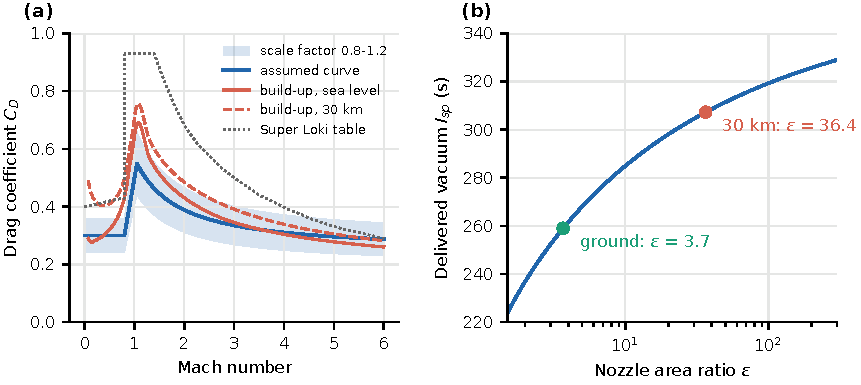
\includegraphics[width=\textwidth]{figures/fig_inputs.pdf}
\caption{Model inputs. (a) Assumed drag coefficient against Mach number with the band covered by the scale factor, the coefficient computed by component build-up for the geometry of Sec.~\ref{sec:traj} at sea level and at 30\,km (unpowered), and the tabulated curve of the Super Loki booster with dart \cite{bollermann1968}. (b) Delivered vacuum specific impulse of UDMH/N$_2$O$_4$ at 2.0\,MPa and $\mathrm{O/F}=2.4$ against nozzle area ratio (92\% of the ideal shifting-equilibrium value). The dots mark the nozzles selected for the baseline vehicle on the ground and at 30\,km.}
\label{fig:inputs}
\end{figure}

\subsection{Vehicle family}
\label{sec:family}

The baseline vehicle has a gross mass $m_0=301.27$\,kg, of which 151.27\,kg is propellant (a propellant fraction of \R{propFrac}), and a diameter of 0.40\,m. For the single-family scaling results the propellant fraction and thrust-to-weight ratio are held fixed and the diameter is scaled as $d\propto m_0^{1/3}$, which keeps the bulk density and fineness constant. For the solid-motor comparators of Sec.~\ref{sec:saving} we use a generic solid motor, modelled as a gas of constant specific-heat ratio 1.16 with a characteristic velocity of 1500$\ms$ and a chamber pressure of 6\,MPa. The ballistic parameter $m_0/A$ then grows as $m_0^{1/3}$; it is \R{betaBase}$\,\mathrm{kg\,m^{-2}}$ for the baseline.

\subsection{Tank and pressurant mass}
\label{sec:tanks}

For the closure study (Sec.~\ref{sec:closure}) the dry mass is written $m_{\mathrm{dry}}=m_{\mathrm{fix}}+f\,m_p$, where $m_{\mathrm{fix}}$ collects everything that does not scale with the propellant mass $m_p$ (engine, airframe, valves, avionics, recovery and payload) and $f$ is the mass of tanks and pressurant system per kilogram of propellant. An ideal thin-walled sphere of volume $V$ at pressure $p$ has a wall mass $\tfrac32\,pV\rho_m/\sigma_a$. We take the allowable stress $\sigma_a$ as the yield strength divided by 1.5, a 5\% ullage, propellant densities of 791 and 1450$\kgm$, and a tank pressure of 3\,MPa for a 2\,MPa chamber. This gives \R{ftAl}\,kg of tank per kilogram of propellant for aluminium 6061-T6 (typical yield 276\,MPa \cite{asm}; the specification minimum is lower, and welds lower the strength further) and \R{ftSS} for stainless steel 321 (yield 205\,MPa \cite{astm}). The tank mass is multiplied by 1.5 to allow for cylindrical sections, welds and fittings.

The pressurant is helium stored at 30\,MPa in an ideal aluminium sphere and expanded adiabatically until the bottle reaches 1.2 times the tank pressure. For an ideal gas the energy balance gives a bottle volume $V_b=\tfrac53\,p_tV_t/(p_i-p_f)$. Per kilogram of propellant this adds \R{heKg}\,kg of helium and \R{heBottleKg}\,kg of bottle. The totals are $f=\R{feedAl}$ for aluminium tanks and $f=\R{feedSS}$ for steel tanks. Helium is treated as an ideal gas. At 290\,K and 30\,MPa its density is 43.57$\kgm$ \cite{nist}, a compressibility factor of \R{heZ}. Enlarging the bottle by that factor raises $f$ for aluminium from \R{feedAl} to \R{feedAlRg} and the gross mass of the 100\,km vehicle of Sec.~\ref{sec:closure} from \R{cBalM} to \R{cBalMRg}\,kg at 30\,km, a small change. The steel-tank case, with more than twice the feed-system mass, bounds the effect of weaker welded aluminium.

A flown stage gives a reference point for $f$. The tank assembly of the Aerobee~150A sustainer, with its helium tank and its helium, weighed \R{abFeed}\,kg per kilogram of propellant, at a tank pressure \R{abTankRatio} times the chamber pressure \cite{busse1966,openaerospace} (Sec.~\ref{sec:aerobee}). Our aluminium estimate is \R{rdAbRatioAl} times that value and our steel estimate \R{rdAbRatioSs} times. The aluminium family is therefore already heavier than flown hardware, and the steel family stands for a much heavier construction. Section~\ref{sec:saving} repeats the comparison with the flown value.

\section{Validation}
\label{sec:validation}

\subsection{Deacon ground firings}

NACA flight-tested the 6.25-inch Deacon solid rocket at Wallops Island and reported, for eight rounds, the gross weight, the total impulse and the maximum velocity measured by Doppler radar \cite{watson1949}. The rounds were launched at an elevation of $70^{\circ}$. We model each round with its reported gross mass and impulse, a propellant mass of \R{deaMp}\,kg (103\,lb), a constant thrust over 2.9\,s (the time of maximum velocity reported for round 6), the 6.75-inch maximum diameter that the report uses for drag, and the drag curve of Fig.~\ref{fig:inputs}(a) with a scale factor of one. The flight path is taken as a straight line at $70^{\circ}$.

Table~\ref{tab:deacon} and Fig.~\ref{fig:validation}(a) compare the computed and measured maximum velocities. For rounds 2--7 the model is high by $\R{deaErrMean}$\% on average and by at most \R{deaErrMaxAbs}\%. Drag removes about \R{deaDragShare}\% of the velocity in these flights, so the comparison does test the drag model. A least-squares fit of the scale factor to rounds 2--7 gives \R{deaCdFit}, inside the 0.8--1.2 band, with an r.m.s. error of \R{deaRmsFit}\%. Rounds 8 and 9, which the report lists at a lower propellant temperature, are over-predicted by $\R{deaErrCold}$\% on average; a colder grain burns for longer than the 2.9\,s we assume for every round.

\subsection{Super Loki Dart}

The Super Loki Dart is a two-part meteorological rocket: a 4-inch booster that burns for 2.0\,s and an unpowered dart that coasts to apogee. The NASA contractor report on the system \cite{bollermann1968} gives the masses (28.32\,kg at launch, 16.87\,kg of propellant, a 6.12\,kg dart), the average sea-level thrust (4450\,lb), tabulated drag coefficients for the two configurations from Mach 0 to 7 or 8, and a computed trajectory for launch at $80^{\circ}$ from sea level. We ran this case with a planar point-mass model, constant thrust, and the report's own drag tables. Our burnout velocity is \R{lokiVb}$\ms$ against the report's \R{lokiVbRep}$\ms$ ($\R{lokiVbErr}$\%), and our apogee is \R{lokiAp}\,km against 113.4\,km ($\R{lokiApErr}$\%). The report's printed trajectory shows a thrust that builds up over the burn, whereas ours is constant. For launch from the elevation of White Sands (1219\,m), where the report states that three flights tracked over apogee reached about 125\,km, the model gives \R{lokiWs}\,km at $80^{\circ}$ ($\R{lokiWsErr}$\%); the launch elevation of those flights is not stated. The model therefore over-predicts this vehicle by about 6\% in apogee.

\subsection{Deacon rockoon flights of 1952--53}

The Naval Research Laboratory's summary of upper-atmosphere rocket firings \cite{smith1954} gives data sheets for the Deacon rockoons flown by the State University of Iowa and by NRL in 1952 and 1953, each with the altitude at which the rocket was fired and the zenith it reached. Nine sheets are complete and legible in the copy we read (Table~\ref{tab:rockoons}); they span firing altitudes of \R{rkFireLo}--\R{rkFireHi}\,km and zeniths of \R{rkObsLo}--\R{rkObsHi}\,km. The first of them, of 28 August 1952, is the flight described by Ludwig \cite{ludwig2004} as the first fully successful rockoon. The sheets do not give the mass of the rocket or its payload; the report quotes a nominal payload of 50\,lb.

We model each flight as a Deacon fired vertically at the stated altitude with the average impulse of the NACA rounds (\R{deaImp}\,kN\,s), and fit one gross mass to each group of flights, since the two groups carried different instruments. For the six Iowa flights the fitted mass is \R{rkSuiMass}\,kg and the r.m.s. error in apogee is \R{rkSuiRms}\%; for the three NRL flights they are \R{rkNrlMass}\,kg and \R{rkNrlRms}\%. Both masses lie in or just above the \R{nacaMassLo}--\R{nacaMassHi}\,kg flown by NACA. Over all nine flights the errors range from $\R{rkWorst}$\% to $\R{rkBest}$\% (Fig.~\ref{fig:validation}b).

The comparison is informative in two ways. The three Iowa flights of 1952, fired between 10.6 and 13.0\,km, are reproduced to \R{rkEarlyRms}\% r.m.s. with a single mass of \R{rkEarlyMass}\,kg. But the model under-predicts the two highest Iowa flights of 1953: the observed apogee rises faster with firing altitude than the computed one. Lighter payloads on those flights would explain it, and so would more drag than we assume, which makes altitude worth more; doubling the drag scale factor lowers the Iowa r.m.s. error to \R{rkSuiCdRms}\%. The records do not let us separate the two. The two drag checks therefore disagree: the ground firings, where velocity was measured directly, fit a scale factor of \R{deaCdFit}, while the rockoon apogees prefer about two. We give more weight to the ground firings, because the rockoon fit is confounded with the unknown payload masses. Section~\ref{sec:gain} gives the attribution of the gain at both scale factors. The model therefore reproduces balloon-launched apogees to about 10\%, with one fitted mass per group, and may understate the benefit of firing altitude for a rocket of high drag.

The fitted masses can be set against one independent value. A secondary compilation lists the Deacon rockoon at 205\,lb (\R{rkAxMass}\,kg) gross with a 37\,lb payload \cite{astronautixdeacon}; we have not found a primary source for it, and it may not apply to every flight. With that mass and no fitting the model over-predicts every flight: by \R{rkAxSuiMean}\% on average for the Iowa flights (r.m.s. \R{rkAxSuiRms}\%) and by \R{rkAxNrlMean}\% for the NRL flights (r.m.s. \R{rkAxNrlRms}\%). To reproduce the Iowa flights with this mass the drag would have to be \R{rkAxCdFit} times our curve (r.m.s. error \R{rkAxCdRms}\%), close to the factor of about two that the fitted-mass comparison prefers and far above the \R{deaCdFit} fitted to the ground firings. The records cannot tell whether the flown rockets were heavier than listed, the drag at altitude higher, or both; higher drag would make the balloon's advantage larger than the model gives. The original accounts \cite{vanallen1954,vanallen1959} may settle this.

\begin{figure}[!htb]
\centering
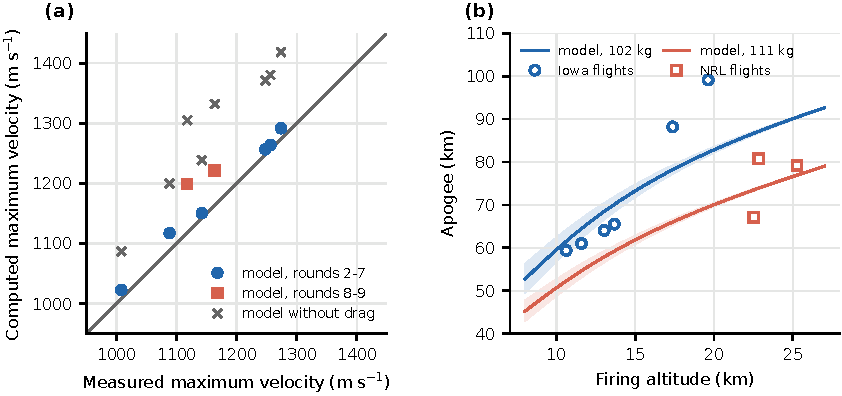
\includegraphics[width=\textwidth]{figures/fig_validation.pdf}
\caption{Validation. (a) Computed against measured maximum velocity for the eight Deacon ground rounds of Ref.~\cite{watson1949}; crosses show the model with drag switched off. (b) Deacon rockoon flights of 1952--53 \cite{smith1954}: zenith against firing altitude (symbols) and the model with one fitted gross mass per group (lines; bands for drag scale factors of 0.8--1.2).}
\label{fig:validation}
\end{figure}

\subsection{Aerobee 150}
\label{sec:aerobee}

The Aerobee~150 is the closest flown relative of the vehicles studied here: a sounding rocket of 0.38\,m diameter whose sustainer is pressure-fed with helium and burns storable hypergolic propellants, inhibited red fuming nitric acid with a mixture of aniline and furfuryl alcohol, at a chamber pressure of \R{abPc}\,MPa and a nozzle area ratio of 4.6, after a solid booster that burns for 2.5\,s. NASA's compendia of Aerobee launchings give its propulsion data, propellant weights and nominal performance \cite{busse1966} and the flights of 1964 with their payload weights and peak altitudes \cite{busse1967}. We took the item-by-item masses from a secondary compilation \cite{openaerospace}, which agrees with the NASA report on the oxidizer weight and on the empty weight.

Two checks follow. The first is of the engine efficiency. By the method of Sec.~\ref{sec:prop}, the ideal shifting-equilibrium specific impulse of these propellants at the published chamber pressure, mixture ratio and area ratio is \R{abIspSlIdeal}\,s at sea level, with a chamber temperature of \R{abTc}\,K and a characteristic velocity of \R{abCstar}$\ms$; the published sea-level thrust and flow rate give \R{abIspSlPub}\,s. The delivered specific impulse of this flown engine is therefore \R{abEtaSl} of the ideal value at sea level and \R{abEtaVac} in vacuum, inside the 0.85--0.95 range of $\eta$ used here and just below the nominal 0.92. The second check is of the trajectory. With the published thrust, flow rate and masses, a vertical flight and the drag curve of Fig.~\ref{fig:inputs}(a), the model departs from the two nominal performances stated in the compendia, for net payloads of 150 and 250\,lb, by $\R{abNomA}$\% and $\R{abNomB}$\% in peak altitude and by $\R{abNomVbA}$\% and $\R{abNomVbB}$\% in burnout velocity (Table~\ref{tab:aerobee}). Four flights from White Sands in 1964 for which the compendium states a net payload weight are over-predicted by \R{abFltLo}--\R{abFltHi}\% in peak altitude, \R{abFltMean}\% on average; their launch angles are not stated, and the model flies them vertically. The comparison supports the trajectory, drag and mass bookkeeping for a pressure-fed liquid vehicle to a few per cent against nominal performance and to about ten per cent against individual flights, the same accuracy as for the solid rockets above. It does not test our UDMH/N$_2$O$_4$ thermochemistry in flight, because the thrust is taken from the report.

\subsection{What the checks do and do not establish}

Table~\ref{tab:valscope} summarises the checks. The first three flight comparisons test the trajectory integration, the drag model at low altitude, the coast to apogee, and, through the rockoon flights, the dependence of apogee on firing altitude, for solid rockets. The Aerobee comparison tests the same bookkeeping for a pressure-fed liquid vehicle and gives a value of the engine efficiency for a flown engine of the class modelled. NASA CEA run directly reproduces our thermochemistry (Sec.~\ref{sec:prop}). RocketPy \cite{rocketpy2021}, an established, independently written flight-dynamics code, flown with the same mass, vacuum thrust, exit area, drag curve and inverse-square gravity, reproduces the baseline apogee to \R{rpGndDiff}\% from the ground and \R{rpBalDiff}\% from 30\,km, in three and in six degrees of freedom; its default environment holds gravity constant above 80\,km, so we tabulated it to 400\,km. None of the checks tests our UDMH/N$_2$O$_4$ engine in flight, the balloon model, flight from a balloon with a mass known from a primary source, or any effect of attitude. The integration itself is converged: tightening the tolerance from $10^{-8}$ to $10^{-11}$ changes the baseline apogees by less than 0.1\,m.

\begin{table}[!htb]
\centering
\caption{Scope of the validation checks.}
\label{tab:valscope}
\footnotesize
\begin{tabular}{@{}>{\raggedright\arraybackslash}p{3.0cm}>{\raggedright\arraybackslash}p{3.1cm}>{\raggedright\arraybackslash}p{4.1cm}>{\raggedright\arraybackslash}p{4.1cm}@{}}
\toprule
Check & Result & Tests & Does not test \\
\midrule
Deacon ground rounds 2--7 \cite{watson1949} & Maximum velocity within \R{deaErrMaxAbs}\% (mean $\R{deaErrMean}$\%) & Impulse and mass bookkeeping; drag to Mach 3.7 near sea level & Coast; high altitude; our generic drag curve above Mach 4 \\
Super Loki Dart \cite{bollermann1968} & Burnout velocity $\R{lokiVbErr}$\%; apogee $\R{lokiApErr}$\% against the report's simulation, about $\R{lokiWsErr}$\% against flights & Planar integration, staging and coast with a published drag table & Our drag curve; thrust history (constant thrust assumed) \\
Nine Deacon rockoons, 1952--53 \cite{smith1954} & Apogee within \R{rkAllRms}\% r.m.s. with one fitted mass per group; \R{rkAxRms}\% r.m.s. with a reported mass and no fit & Balloon-launched apogee and its dependence on firing altitude & Absolute level (reported mass from a secondary source); launch angle unknown \\
Aerobee~150 \cite{busse1966,busse1967} & Nominal peak altitudes within \R{abNomMax}\%; \R{abFltN} flights over-predicted by \R{abFltLo}--\R{abFltHi}\%; delivered specific impulse \R{abEtaVac} of ideal & Trajectory, drag and mass bookkeeping for a pressure-fed liquid vehicle; efficiency of a flown engine of the same class & Our propellants; launch angle of the flights (vertical assumed); item masses from a secondary compilation \\
NASA CEA \cite{cea2026} & Specific impulse and $c^{*}$ within \R{ceaMaxDiff}\% & Our thermochemistry, shifting and frozen & Engine efficiency $\eta$; combustion and nozzle losses \\
RocketPy \cite{rocketpy2021} & Baseline apogees within \R{rpMaxDiff}\%, 3 and 6 degrees of freedom & Integration, atmosphere, gravity and pressure thrust, independently coded & Physics common to both codes (drag curve, constant thrust) \\
\bottomrule
\end{tabular}
\end{table}

\section{The float altitude that minimises the launched mass}
\label{sec:general}

\subsection{Closure for a 100\,km apogee}
\label{sec:closure}

A pressure-fed vehicle has to carry tanks and pressurant whose mass grows with the propellant load (Sec.~\ref{sec:tanks}). We therefore fix the target, a 100\,km apogee, and solve for the propellant mass that reaches it, with $m_{\mathrm{dry}}=m_{\mathrm{fix}}+f\,m_p$ and the diameter scaled with the gross mass as in Sec.~\ref{sec:family}.

Figure~\ref{fig:closure} and Table~\ref{tab:closure} give the result. With $m_{\mathrm{fix}}=80$\,kg and aluminium tanks, a ground-launched vehicle needs \R{cGndMp}\,kg of propellant and has a gross mass of \R{cGndM}\,kg. Ignited at 30\,km it needs \R{cBalMp}\,kg of propellant, a dry mass of \R{cBalDry}\,kg and a gross mass of \R{cBalM}\,kg: \R{cPropRatio} times less propellant and \R{cMassRatio} times less vehicle. It produces \R{cBalF}\,kN for \R{cBalTb}\,s. With steel tanks the ground-launched vehicle grows to \R{cGndMSS}\,kg, while the balloon-launched one is \R{cBalMSS}\,kg. The balloon makes the design much less sensitive to tank mass.

The balloon is not free. For the aluminium vehicle at 30\,km it has a volume of \R{cBalV}\,m$^3$, an envelope of \R{cBalEnv}\,kg and \R{cBalGas}\,kg of hydrogen at float. Rocket, gondola, envelope and launch gas together come to about \R{cSysBal}\,kg, not far below the \R{cGndM}\,kg of the ground-launched vehicle. At 20\,km the vehicle is \R{cTwentyM}\,kg and the balloon only \R{cTwentyV}\,m$^3$. Most of the saving is available well below 30\,km.

\begin{figure}[!htb]
\centering
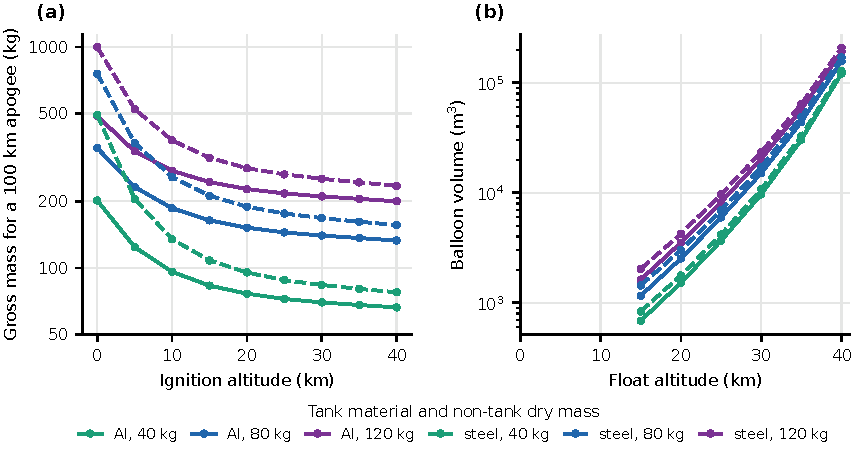
\includegraphics[width=\textwidth]{figures/fig_closure.pdf}
\caption{Self-consistent vehicles that reach 100\,km, for 3\,MPa tanks of aluminium 6061-T6 (solid) or stainless steel 321 (dashed) and three values of the non-tank dry mass. (a) Gross mass against ignition altitude. (b) Volume of the hydrogen balloon that carries the vehicle and a 30\,kg gondola.}
\label{fig:closure}
\end{figure}

\subsection{The float altitude that minimises launched mass}
\label{sec:optimum}

Section~\ref{sec:closure} compared rockets. What has to be lifted off the ground, however, is the rocket together with its gondola, envelope and gas. For each of fourteen vehicle families (aluminium or steel tanks, $m_{\mathrm{fix}}$ from 10 to 640\,kg) we closed the vehicle for a 100\,km apogee at float altitudes from 0 to 40\,km and added a gondola of 10\% of the rocket mass, the envelope, and the hydrogen with 10\% free lift.

The total launched mass has a minimum (Fig.~\ref{fig:optimum}a, Table~\ref{tab:optimum}). It lies between \R{zsLo} and \R{zsHi}\,km for every family, although the ground-launched mass of these families spans \R{zsMassLo} to \R{zsMassHi}\,kg. At the optimum the launched mass is \R{zsSaveLo}--\R{zsSaveHi}\% below that of a ground-launched rocket of the same design; Sec.~\ref{sec:saving} shows that this saving, unlike the location of the optimum, does not survive a fair comparison. The minimum is flat: a float altitude between \R{zsBandLo} and \R{zsBandHi}\,km is within 5\% of the optimum for all fourteen families. For aluminium vehicles with $m_{\mathrm{fix}}$ up to 80\,kg the balloon system becomes heavier than the ground-launched rocket above 32--35\,km; for larger vehicles and for steel tanks the crossing lies at 37.5\,km or beyond. Targets of 60 and 150\,km give optima in the same range (Fig.~\ref{fig:optimum}b).

For the vehicle of Sec.~\ref{sec:closure} ($m_{\mathrm{fix}}=80$\,kg, aluminium) the interpolated optimum is at \R{zsBase}\,km. At the nearest computed altitude, \R{zsBaseGrid}\,km, a \R{zsBaseRocket}\,kg rocket and a \R{zsBaseV}\,m$^3$ balloon make a launched mass of \R{zsBaseTotGrid}\,kg, against \R{zsBaseGnd}\,kg from the ground.

The result is not sensitive to the balloon assumptions. For the same vehicle, envelope areal densities of 20 and 40\,$\mathrm{g\,m^{-2}}$ move the optimum to \R{zsSigLo} and \R{zsSigHi}\,km, and gondola fractions of 5\% and 20\% to \R{zsGonLo} and \R{zsGonHi}\,km, with savings of \R{zsGonLoSave}\% and \R{zsGonHiSave}\% (envelope densities of 20 and 40\,$\mathrm{g\,m^{-2}}$ give \R{zsSigLoSave}\% and \R{zsSigHiSave}\%). Over all twelve such variations for $m_{\mathrm{fix}}=20$, 80 and 320\,kg the optimum stays between \R{zsVarLo} and \R{zsVarHi}\,km.

The two envelope laws differ in how the optimum moves with size. With the film law it rises slowly, by about \R{zsSlope}\,km per decade of mass for the aluminium family. With the fitted law the optimum is \R{grFitZLo}--\R{grFitZHi}\,km and it falls with size: it is \R{grFitAlSmall}\,km for the smallest aluminium family and \R{grFitAlLarge}\,km for the largest. Section~\ref{sec:analytic} explains both trends. A third law, $\sigma S+k\,m_s$, in which the second term stands for load tapes and film that are sized by the suspended load and not by the area, behaves like the film law. For $k=0.05$, 0.10 and 0.20 the optimum stays at \R{zsKlALo}--\R{zsKlAHi}, \R{zsKlBLo}--\R{zsKlBHi} and \R{zsKlCLo}--\R{zsKlCHi}\,km and the slope at \R{zsKlASlope}, \R{zsKlBSlope} and \R{zsKlCSlope}\,km per decade, while the smallest saving falls from \R{zsSaveLo}\% to \R{zsKlCSaveLo}\%. A term proportional to the load raises the launched mass at every altitude by nearly the same factor, so it lowers the saving but not the location of the optimum. We have no measured value of $k$ for zero-pressure balloons of this size, so these values are a sensitivity range, not an estimate.

The propellant must also survive the ascent. Nitrogen tetroxide freezes at about $-11\,^\circ$C, and the tropopause is near $-56\,^\circ$C. We sized a foam jacket (conductivity 0.03\,W\,m$^{-1}$\,K$^{-1}$, density 35$\kgm$) around two spherical tanks so that propellant loaded at 20\,$^\circ$C cools by no more than 25\,K during an ascent at 5\,m\,s$^{-1}$ and half an hour at float, taking the outside of the foam at the local air temperature and the propellant at its initial temperature, which overstates the heat loss. The required thickness is at most \R{insThickReq}\,mm; with a practical minimum of 25\,mm the jacket weighs \R{insBase}\,kg for the baseline vehicle, \R{insFracLo}--\R{insFracHi}\% of the rocket mass across the families. Carried by the gondola and released at ignition, it moves the optimum by less than \R{zsThShift}\,km. Radiative loss to a cold sky is not included and would need a test.

The smallest families need balloons of a few hundred cubic metres, a size that could be flown on latex balloons or clusters of them, as Okninski \emph{et al.} \cite{okninski2016} proposed; Sec.~\ref{sec:analytic} treats that case. The optimum found here is close to the altitude of about 15\,km above which Sarigul-Klijn \emph{et al.} \cite{sarigul2005} saw little further velocity gain for an orbital vehicle with a fixed nozzle, although their result did not include the mass of a carrier.

\begin{figure}[!htb]
\centering
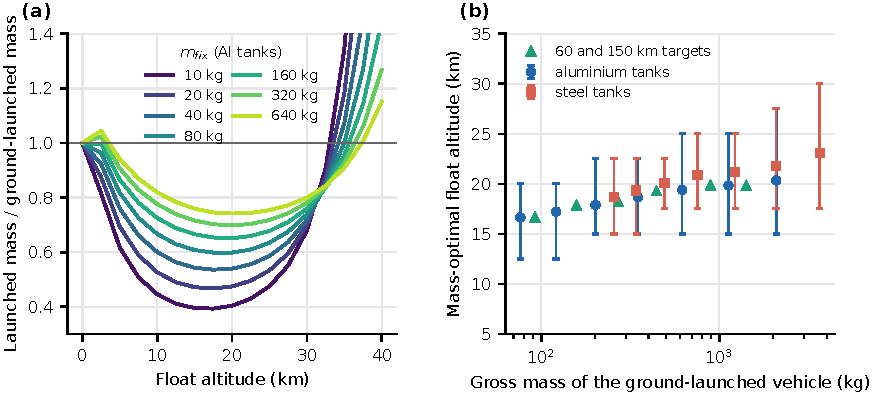
\includegraphics[width=\textwidth]{figures/fig_optimum.pdf}
\caption{(a) Total launched mass (rocket, gondola, envelope and hydrogen) for a 100\,km apogee, divided by the mass of the ground-launched rocket, against float altitude, for aluminium tanks. (b) Float altitude of minimum launched mass against the mass of the ground-launched vehicle. Bars show the range within 5\% of the minimum.}
\label{fig:optimum}
\end{figure}

\begin{table}[!htb]
\centering
\caption{Mass-optimal float altitude for a 100\,km apogee: ground-launched gross mass, interpolated optimum altitude $z^{*}$, and the launched mass, rocket mass and balloon volume at the nearest computed altitude $z_g$.}
\label{tab:optimum}
\small
\begin{tabular}{cccccccc}
\toprule
Tanks & $m_{\mathrm{fix}}$ & Ground-launched & $z^{*}$ & $z_g$ & Launched mass & Rocket & Balloon \\
 & (kg) & mass (kg) & (km) & (km) & (kg) & (kg) & (m$^3$) \\
\midrule
\tabin{tab_optimum.tex}
\bottomrule
\end{tabular}
\end{table}

\subsection{The envelope rule}
\label{sec:analytic}

The location of the optimum and the size of the saving respond so differently to the assumptions that the reason is worth making explicit, and it can be made exact for any balloon. Let the envelope mass be any function $m_e=E(V,m_s)$ of the volume and of the suspended mass $m_s$ (rocket and gondola). Let the balloon displace $\ell$ times the mass it carries, so that $V\Delta\rho(z)=\ell\,(m_s+m_e)$, where the net lift per unit volume $\Delta\rho$ is proportional to the air density; $\ell=1$ for a balloon at float and $\ell>1$ for one that is still rising with free lift. Let the quantity to be minimised be
\begin{equation}
J=m_s+\mu\,m_e ,
\label{eq:objective}
\end{equation}
where $\mu$ is the price of a kilogram of envelope relative to a kilogram of suspended mass. With $\mu=1$, $J$ is the launched mass divided by the constant $1+1.1\chi$, where $\chi=M_g/(M_a-M_g)$ is the gas mass per kilogram lifted. Write
\begin{equation}
\phi=\frac{m_e}{m_s},\qquad \Lambda=\frac{m_s}{|dm_s/dz|},\qquad \alpha=\frac{\partial\ln E}{\partial\ln V},\qquad \beta=\frac{\partial\ln E}{\partial\ln m_s}
\end{equation}
for the envelope fraction, the altitude over which the suspended mass would fall by its own amount at the local rate, and the two exponents of the envelope law, and $H_\rho=-\rho/(d\rho/dz)$ for the local density scale height. The buoyancy balance gives $d\ln V/dz=1/H_\rho+d\ln(m_s+m_e)/dz$, and the envelope law gives $dm_e/dz=m_e\,(\alpha\,d\ln V/dz+\beta\,d\ln m_s/dz)$. Eliminating $V$ and setting $dJ/dz=0$,
\begin{equation}
\frac{1}{\Lambda}\left[1+\mu\beta\phi+(\mu-1)\frac{\alpha\phi}{1+\phi}\right]=\frac{\mu\,\alpha\,\phi}{H_\rho}.
\label{eq:general}
\end{equation}
For the launched mass ($\mu=1$) this is
\begin{equation}
\phi^{*}=\frac{1}{\alpha\Lambda/H_\rho-\beta},\qquad\text{that is,}\qquad \alpha\,m_e=H_\rho\left|\frac{dm_s}{dz}\right|(1+\beta\phi)\quad\text{at }z^{*}.
\label{eq:rule}
\end{equation}
At the mass-optimal float altitude the envelope is a fixed fraction of the suspended mass, set by the ratio of two lengths and by two exponents. For the film law ($\alpha=\tfrac23$, $\beta=0$) it reads $m_e=\tfrac32H_\rho\,|dm_s/dz|$: the envelope weighs as much as the suspended mass that the last $\tfrac32H_\rho\approx9.5$\,km of altitude saved. For an envelope that is a sum of power-law terms, $\alpha$ and $\beta$ are the means over the terms weighted by their masses; for the fitted law, with terms $m_A$ and $m_L$, Eq.~(\ref{eq:rule}) reads $\tfrac23m_A+\tfrac13m_L=H_\rho\,|dm_s/dz|\,(1+b\,V^{1/3})$.

Equation~(\ref{eq:general}) is exact. It uses nothing about the rocket except its closed mass and the slope of that mass against float altitude, and nothing about the ground-launched comparator. The lift gas and the free lift change the volume but not the form of the condition. Solved on the rocket curves described next, it agrees with direct minimisation of $J$ to \R{grResid} significant figures for every family, for the four envelope laws of Table~\ref{tab:laws} and for prices $\mu$ from 0.03 to \R{grMuMax}. The one exception is an optimum that falls on an altitude at which the lapse rate of the standard atmosphere changes (20 and 32\,km): $H_\rho$ is discontinuous there, and the condition holds between its two one-sided values.

\emph{A one-step estimate.} To see what sets $z^{*}$, let $\mathcal{R}(z)$ be the left side of Eq.~(\ref{eq:general}) divided by the right side; it is above one below the optimum and equal to one at it. The closed rocket mass is well approximated by $m_r(z)=m_\infty+B\,e^{-z/L}$, which fits every family between 10 and 35\,km to within \R{anFitResid}\% with $L=\R{anLLo}$--\R{anLHi}\,km, so the saving side falls as $e^{-z/L}$. The envelope side grows as $e^{\alpha_2z/H_\rho}$, where $\alpha_2$ is the mean of $\alpha$ over the terms weighted by $\alpha_im_i$ and equals $\alpha$ for a single power law. Hence $\ln\mathcal{R}$ is nearly linear in altitude (Fig.~\ref{fig:general}a), and from any trial altitude $z_t$
\begin{equation}
z^{*}\approx z_t+L_{\mathrm{eff}}\ln\mathcal{R}(z_t),\qquad L_{\mathrm{eff}}=\left(\frac{1}{L}+\frac{\alpha_2}{H_\rho}\right)^{-1}.
\label{eq:zstar}
\end{equation}
$L_{\mathrm{eff}}$ is \R{grAreaLeffLo}--\R{grAreaLeffHi}\,km for the film law and \R{grFitLeffLo}--\R{grFitLeffHi}\,km for the fitted law. A designer therefore needs one trial design: the suspended mass at two or three altitudes, which gives $\Lambda$ and $L$, and the envelope that carries it at one of them. From a trial altitude of 20\,km, one step of Eq.~(\ref{eq:zstar}) lands within \R{grStepOne}\,km of the exact optimum for every family and law of Table~\ref{tab:laws} (Fig.~\ref{fig:general}c), and a second step within \R{grStepTwo}\,km. Against the optimum of the full model, found on the 2.5\,km altitude grid, Eq.~(\ref{eq:general}) with the fitted rocket curves is within \R{grAreaDiff}\,km for the film law and \R{grFitDiff}\,km for the fitted law (Table~\ref{tab:laws}; Table~\ref{tab:analytic} gives the film law family by family).

\begin{table}[!htb]
\centering
\caption{The envelope rule for four envelope laws over the fourteen families: exponents $\alpha$ and $\beta$ at the optimum, optimum $z^{*}$ of the full model on the altitude grid, largest difference between it and Eq.~(\ref{eq:general}) solved on the fitted rocket curves, envelope fraction $\phi^{*}$ and $L_{\mathrm{eff}}$ at the optimum, and the trend of the optimum with the ground-launched mass (aluminium families, km per decade of mass).}
\label{tab:laws}
\small
\begin{tabular}{@{}>{\raggedright\arraybackslash}p{4.2cm}ccccccc@{}}
\toprule
Envelope law & $\alpha$ & $\beta$ & $z^{*}$ & Rule, model & $\phi^{*}$ & $L_{\mathrm{eff}}$ & Trend \\
 & & & (km) & differ by (km) & (\%) & (km) & \\
\midrule
\tabin{tab_general.tex}
\bottomrule
\end{tabular}
\end{table}

\begin{figure}[!htb]
\centering
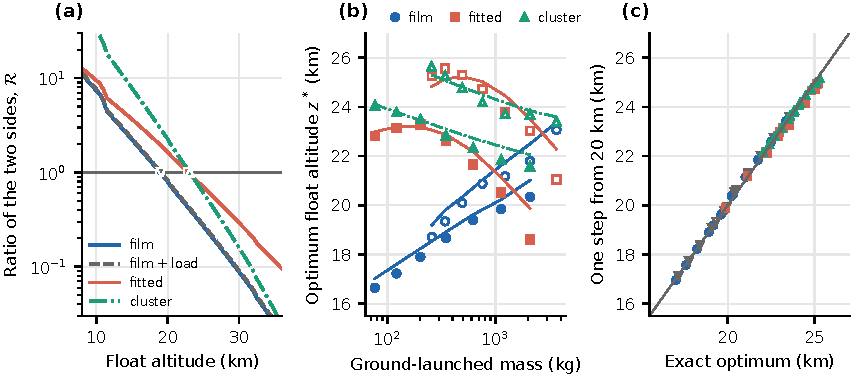
\includegraphics[width=\textwidth]{figures/fig_general.pdf}
\caption{The envelope rule. (a) Ratio $\mathcal{R}$ of the saving side of Eq.~(\ref{eq:general}) to its envelope side against float altitude, for the family with $m_{\mathrm{fix}}=80$\,kg and aluminium tanks and four envelope laws; the optimum is where $\mathcal{R}=1$, and each line has a slope close to $-1/L_{\mathrm{eff}}$. (b) Optimum of the full model against the ground-launched mass for three envelope laws (symbols; filled for aluminium, open for steel tanks) and Eq.~(\ref{eq:general}) on the fitted rocket curves (lines). (c) One step of Eq.~(\ref{eq:zstar}) from a trial altitude of 20\,km against the exact optimum, for all families and laws.}
\label{fig:general}
\end{figure}

Five consequences follow.

\emph{Every input enters through a logarithm.} Multiplying the envelope law by a factor $k$ moves the optimum by $-L_{\mathrm{eff}}\ln k$. Doubling the areal density of the film law lowers it by \R{grDblAreaPred}\,km for the baseline family (direct minimisation \R{grDblAreaExact}\,km; the full model \R{anSigModel}\,km), and doubling both coefficients of the fitted law by \R{grDblFitPred}\,km (\R{grDblFitExact}\,km). Scaling the suspended mass by a factor, as a heavier gondola does, moves the optimum by $L_{\mathrm{eff}}\,(1-\alpha-\beta)$ times the logarithm of the factor: raising the gondola from 5\% to 20\% of the rocket mass raises the film-law optimum by \R{grGonAreaPredAbs}\,km (full model \R{anGonModel}\,km).

\emph{The comparator does not enter.} The ground-launched rocket appears nowhere in Eq.~(\ref{eq:general}). A better ground comparator cannot move the optimum; it can only change the saving.

\emph{The saving is linear in what the optimum feels only logarithmically.} At the optimum the launched mass is $(1+1.1\chi)(1+\phi^{*})\,m_s(z^{*})$, which scales directly with the gondola fraction, the envelope law and the rocket's dry structure, while the ground-launched mass is set by the propellant needed to fight drag from sea level. A 20\% change in any of these inputs moves the optimum by less than a kilometre and the saving by many percentage points. Section~\ref{sec:saving} finds exactly this.

\emph{The sign of the size trend is the sign of $1-\alpha-\beta$.} If the vehicle is scaled up at fixed $\Lambda$, the envelope side of Eq.~(\ref{eq:rule}) scales as $m_s^{\alpha+\beta}$ and the saving side as $m_s$. An envelope whose mass grows more slowly than the load it lifts ($\alpha+\beta<1$) gives large systems an economy of scale and a higher optimum; one that grows faster reverses it. The film law has $\alpha+\beta=\tfrac23$, and its optimum rises by \R{zsSlope}\,km per decade of mass. In the fitted law the load-bearing term has $\alpha+\beta=\tfrac43$; at the optimum $\alpha+\beta$ runs from \R{grFitSumLo} for the smallest family to \R{grFitSumHi} for the largest, and the optimum falls by \R{grFitSlopeAbs}\,km per decade (\R{grOwnFitAlSlopeAbs}\,km per decade when each vehicle is designed for its own launch, Sec.~\ref{sec:saving}). Relative to the film law, the fitted law therefore moves the optimum by between $\R{grFitShiftLo}$ and $\R{grFitShiftHi}$\,km, up for small vehicles and down for the largest (Fig.~\ref{fig:general}b). The rocket adds a weaker trend of its own: a large vehicle loses relatively less to drag, which lowers the optimum, and its saving decays more slowly with altitude, which raises it. Whether the optimum rises or falls with size is therefore decided mainly by the balloon.

\emph{A price on the balloon moves the optimum by a bounded amount.} A price $\mu$ shifts the optimum by about $-L_{\mathrm{eff}}\ln\mu$. If the envelope, the gondola and the gas are all priced at $r$ times the rocket per kilogram, as in the cost test of Sec.~\ref{sec:saving}, then $\mu=r\,(1+1.1\chi)(1+f_g)/[1+rf_g+1.1\chi r(1+f_g)]$, where $f_g$ is the gondola fraction, because the gondola and the gas scale with the suspended mass and are charged at the same rate. With these values of $\mu$ Eq.~(\ref{eq:general}) reproduces the cost-optimal altitudes of the full model to within \R{grCostMed}\,km (median; \R{grCostDiff}\,km at worst, where the best design changes between grid altitudes). As $r$ grows without limit $\mu$ tends to $(1+1.1\chi)(1+f_g)/[f_g+1.1\chi(1+f_g)]$, which is \R{grMuMax} for a 20\% gondola. However expensive the balloon system, the cost-optimal altitude is therefore at most \R{grInfFallLo}--\R{grInfFallHi}\,km below the mass-optimal one, at \R{grInfZLo}--\R{grInfZHi}\,km. In the other direction, an envelope that is cheap beside the rocket raises the optimum until the balloon's ceiling stops it.

\emph{Other balloons.} The rule is not tied to zero-pressure film balloons. A latex sounding balloon rises until it bursts at a volume fixed by its size. The catalogue burst diameters of \R{ltxN} balloons of 350--4000\,g \cite{kaymont} follow $m_e=c\,V_b^{\alpha}$ with $\alpha=\R{ltxAlpha}$ (r.m.s. \R{ltxRms}\%). That is close to the film law with only \R{ltxArealLo}--\R{ltxArealHi}\,g\,m$^{-2}$ at burst, but the largest of these balloons reaches \R{ltxVHi}\,m$^3$, enough for only the \R{ltxFits} smallest families. Larger loads need a cluster of identical balloons, each filled to burst at the firing altitude, and for a cluster the envelope mass is proportional to the volume: $\alpha=1$ and $\beta=0$. Equation~(\ref{eq:rule}) then gives $m_e=H_\rho\,|dm_s/dz|$, an $L_{\mathrm{eff}}$ of only \R{grCluLeffLo}--\R{grCluLeffHi}\,km, no dependence on the gondola fraction and, because $\alpha+\beta=1$, no economy of scale: for clusters of \R{cluKg}\,kg balloons the optimum is \R{grCluZLo}--\R{grCluZHi}\,km and falls by \R{grCluSlopeAbs}\,km per decade of mass. Latex is also cheap beside a rocket. With the envelope priced at a tenth of the suspended mass per kilogram the cluster optimum is \R{grCluTenthLo}--\R{grCluTenthHi}\,km, and at $\mu=0.03$ it is \R{grCluCheapLo}--\R{grCluCheapHi}\,km, close to the ceiling of \R{cluCeil}\,km at which such a balloon lifts only itself. This is the regime of Okninski \emph{et al.} \cite{okninski2016}, who used clusters of commercial latex balloons, found that the rocket and not the balloon drove the cost, and concluded that the highest launch altitude they considered was best. Their result and ours are then consistent: the same condition, evaluated for a different envelope law and a different price. Material that is sized by pressure behaves differently again: a shell or tendons that hold a superpressure proportional to the ambient pressure have a mass proportional to $p(z)V$, which at a given temperature is a fixed fraction of the lift, so they add no term that grows with altitude.

In summary, the float altitude of least launched mass can be found without a system model.
\begin{enumerate}
\item Close the rocket for the target at two or three float altitudes. This gives the suspended mass $m_s$, its slope and hence $\Lambda$, and the decay length $L$ of the slope (\R{anLLo}--\R{anLHi}\,km here).
\item For the balloon that carries $m_s$ at one of these altitudes, find the envelope fraction $\phi$ and the exponents $\alpha$ and $\beta$ of its mass law (Table~\ref{tab:laws}).
\item Compare $\phi$ with $\phi^{*}=1/(\alpha\Lambda/H_\rho-\beta)$. If the envelope is a larger fraction of the suspended mass than this, the trial altitude is too high, and Eq.~(\ref{eq:zstar}) gives the correction.
\end{enumerate}

\subsection{Altitudes that programmes have chosen}
\label{sec:programmes}

Table~\ref{tab:programmes} lists the firing altitudes of rockoon programmes for which we found a stated value. The comparison is suggestive, not a test: altitude is chosen for range safety, balloon availability and cost as well as mass, and the recent entries are statements by companies or in the press. With that caution, most of them lie in or near the band of \R{zsLo}--\R{grFitZHi}\,km spanned by the two envelope laws: the Deacon rockoons of 1952--53, Leo Aerospace (18\,km), AstroX (about 20\,km), Bloostar (20--25\,km) and the flight test of B2Space (21.5\,km); ARCA fired at 14\,km and planned 18\,km. Three chose 30--35\,km. Far Side, a four-stage solid vehicle designed to be fired through its balloon at 24--30\,km, sought the highest possible apogee, not the least mass, and its balloon was heavy by the standard of Table~\ref{tab:laws}: a \R{fsEnv}\,kg envelope of \R{fsVol}\,m$^3$ for a suspended load of \R{fsLoad}\,kg \cite{farside}, an envelope fraction of \R{fsPhi}\% against \R{grAreaEpsLo}--\R{grAreaEpsHi}\% at the optimum of the film law. Part of the difference is the thicker film of the time. The other two, SpaceRyde and the operational B2Space system, are orbital launchers. A rocket that is far dearer per kilogram than its balloon is the case in which Sec.~\ref{sec:analytic} predicts a higher optimum, although Bloostar, also an orbital launcher, states 20--25\,km.

\begin{table}[!htb]
\centering
\caption{Firing altitudes of rockoon programmes and studies. ``Flown'' entries are altitudes at which a rocket was fired; the others are stated designs.}
\label{tab:programmes}
\small
\begin{tabular}{@{}>{\raggedright\arraybackslash}p{4.9cm}>{\raggedright\arraybackslash}p{4.4cm}>{\raggedright\arraybackslash}p{4.6cm}@{}}
\toprule
Programme & Vehicle & Firing altitude (km) \\
\midrule
State University of Iowa and NRL, 1952--53 \cite{smith1954} & Deacon solid rocket, about 100\,kg & \R{rkFireLo}--\R{rkFireHi} (flown, nine flights of Table~\ref{tab:rockoons}) \\
Far Side, 1957 \cite{farside} & Four-stage solid, 0.9\,t & 24--30 (design) \\
ARCA Helen~2, 2010 \cite{arca2010} & Suborbital demonstrator & 14 (flown); 18 planned for a larger system \\
Zero 2 Infinity Bloostar \cite{eoportal} & Methane and oxygen, 4.9\,t, to orbit & 25 (flown, prototype, 2017); 20--25 design \\
Leo Aerospace \cite{purdue2018} & Small-satellite launcher & 18 (design) \\
SpaceRyde \cite{ansys2021} & Small-satellite launcher & 30 (design) \\
B2Space \cite{b2space,parsonson2025} & Solid rocket; orbital system planned & 21.5 (flown, 2025); 35 for the orbital system \\
AstroX \cite{jiji2024} & Small suborbital rocket & about 20 (design) \\
Janhunen \emph{et al.} \cite{janhunen2018} & 10\,t rocket under a steam balloon & 18 (study) \\
Okninski \emph{et al.} \cite{okninski2016} & Small solid rocket, latex cluster & 20--40 studied; highest found best \\
\bottomrule
\end{tabular}
\end{table}

\section{Whether a rockoon saves mass}
\label{sec:saving}

The saving of Sec.~\ref{sec:optimum} is measured against a ground-launched vehicle with the same thrust-to-weight ratio, nozzle rule and proportions as the balloon-launched one, and it ignores hardware that only a rockoon needs. We remove both simplifications here.

\emph{Comparators designed for their own launch.} Each ground-launched family was closed again for every combination of fineness 8--25, thrust-to-weight ratio 1.5--6 and ground exit pressure down to 0.4 of ambient, a typical separation limit \cite{sutton2017}, and each balloon-launched family at every float altitude for fineness 8--15 and thrust-to-weight ratio 2--6. Every best ground vehicle takes the slimmest body allowed, a fineness of 25, with a thrust-to-weight ratio of \R{dsGndTwLo}--\R{dsGndTwHi} and an exit pressure of \R{dsGndSepLo}--\R{dsGndSepHi} of ambient; these vehicles are \R{dsRedLo}--\R{dsRedHi}\% lighter than the same-design ones. The generic drag coefficient does not grow with fineness, so the model rewards slenderness; a fineness of 30 or 35 would lower the ground-launched mass by a further \R{slimThirtyLo}--\R{slimThirtyHi}\% or \R{slimThirtyFiveLo}--\R{slimThirtyFiveHi}\% (three families checked), and the savings below by about as much. We stop at 25 because longer bodies need structure and fin area that the model does not count, and test the effect of the wetted area below. Without any rockoon-only hardware the optimum is then \R{scNoneZLo}--\R{scNoneZHi}\,km and the saving \R{scNoneSaveLo}--\R{scNoneSaveHi}\%.

\emph{Hardware that only a rockoon needs.} Its divergent nozzle section is larger: at 30\,km the baseline nozzle, a $15^{\circ}$ cone filling the 0.40\,m base, is \R{skBaseL}\,m long and weighs about \R{skBaseM}\,kg at an assumed 10\,kg\,m$^{-2}$ of wall, against \R{skGndL}\,m and \R{skGndM}\,kg on the ground; we add the divergent-section mass to every vehicle and close it again. A rocket hanging under a balloon also needs a launcher and attitude control or spin-up, since fins do nothing at near-zero dynamic pressure, which we represent by a heavier gondola, and the envelope may carry load tapes sized by the load ($k$ of Sec.~\ref{sec:optimum}). In a central case (a 10\,kg\,m$^{-2}$ nozzle wall, a gondola of 20\% of the rocket mass and $k=0.1$) the optimum is \R{scCentralZLo}--\R{scCentralZHi}\,km and the saving is \R{scCentralSsLo}--\R{scCentralSsHi}\% for steel tanks and \R{scCentralAlLo} to \R{scCentralAlHi}\% for aluminium tanks. In the most pessimistic case we tried (20\,kg\,m$^{-2}$, 30\% and $k=0.2$ together) the optimum is \R{scWorstZLo}--\R{scWorstZHi}\,km, the saving for steel tanks is \R{scWorstSsLo}--\R{scWorstSsHi}\%, and for aluminium tanks it is \R{scWorstAlLo} to \R{scWorstAlHi}\%, negative for every family.

\emph{The fitted envelope law.} With the fitted law of Eq.~(\ref{eq:envfit}) and the central hardware penalties the optimum is \R{scFittedZLo}--\R{scFittedZHi}\,km and the saving is \R{scFittedSsLo}--\R{scFittedSsHi}\% for steel and \R{scFittedAlLo} to \R{scFittedAlHi}\% for aluminium tanks. Family by family the optimum moves by between $\R{grCenShiftLo}$ and $\R{grCenShiftHi}$\,km relative to the film law, up for the small families and down for the largest, as Sec.~\ref{sec:analytic} predicts: the fitted envelope is lighter than the film law for small loads and heavier for large ones.

\emph{Two-stage and solid-motor comparators.} A sounding rocket that reaches 100\,km from the ground is usually staged or solid. We closed two-stage pressure-fed vehicles with the same engine model, in which the booster carries a fixed mass of \R{betaLiq}\,$m_{\mathrm{fix}}$ for its engine, valves and structure, the second-stage nozzle is chosen for the staging altitude and carries its divergent-section mass, and the split of propellant, the two thrust-to-weight ratios and the fineness are optimised. They are \R{tsLiqRatioLo}--\R{tsLiqRatioHi} times the mass of the best single-stage vehicle: lighter for all seven steel-tank families, where staging drops heavy tanks early, and heavier for all seven aluminium-tank families, where the booster's own engine and valves cost more than staging saves. Against the lighter of the two ground options, the rockoon with the central penalties saves \R{liqBestSaveSsLo}--\R{liqBestSaveSsHi}\% for steel tanks and \R{liqBestSaveAlLo} to \R{liqBestSaveAlHi}\% for aluminium tanks. For solid motors we used the generic motor of Sec.~\ref{sec:model} with \R{fSolid}\,kg of case, liner and nozzle per kilogram of propellant, a non-propulsive mass $m_{\mathrm{fix}}$, and a booster fixed mass of \R{betaSol}\,$m_{\mathrm{fix}}$. Two-stage solid vehicles are \R{tsSolRatioLo}--\R{tsSolRatioHi} times the mass of the best single-stage solid vehicle. A solid rockoon with the central penalties has its optimum at \R{solZLo}--\R{solZHi}\,km and saves \R{solSaveLo} to \R{solSaveHi}\% against the better of the two. Table~\ref{tab:comparators} collects the comparators.

\emph{Flown dry masses.} The tank and motor masses above are estimates, and two published values test them. The Aerobee~150A sustainer carried \R{rdAbF}\,kg of tanks and pressurant per kilogram of propellant (Sec.~\ref{sec:tanks}), less than our aluminium estimate. A family with this value, designed and compared in the same way, has its optimum at \R{rdAbZLo}--\R{rdAbZHi}\,km and saves \R{rdAbSaveLo} to \R{rdAbSaveHi}\% against the lighter of the one- and two-stage ground vehicles; the rockoon is the heavier option for \R{rdAbNeg} of the seven sizes. For solid motors, the generic \R{fSolid}\,kg of inert mass per kilogram of propellant corresponds to a motor mass fraction of 0.87. The hardware of the Super Loki booster, fins included, weighed \R{rdSolSlF}\,kg per kilogram of its propellant \cite{bollermann1968}. With that value a two-stage vehicle is the lighter ground option for all seven sizes, and the solid rockoon has its optimum at \R{rdSolSlZLo}--\R{rdSolSlZHi}\,km and saves \R{rdSolSlSaveLo}--\R{rdSolSlSaveHi}\%, against \R{solSaveLo} to \R{solSaveHi}\% with the generic motor. Lighter liquid tanks lower the saving and a heavier solid motor raises it, which is the dependence on dry structure found above.

\emph{Drag that grows with fineness.} Because the generic drag curve does not charge a slender body for its wetted area, we repeated the design search with the skin-friction term of the component build-up of Sec.~\ref{sec:traj}, evaluated for each body's own fineness and added to the generic curve as its difference from the value at a fineness of 10. Every best ground vehicle still takes the slimmest body allowed, but it is \R{rdFdHeavyLo}--\R{rdFdHeavyHi}\% heavier than with the generic curve, while the rockoon changes by at most \R{rdFdRkHeavyHi}\%. Against the lighter of the one- and two-stage ground vehicles the saving becomes \R{rdFdSaveSsLo}--\R{rdFdSaveSsHi}\% for steel and \R{rdFdSaveAlLo} to \R{rdFdSaveAlHi}\% for aluminium tanks, \R{rdFdGainAlLo}--\R{rdFdGainAlHi} points more than before for aluminium, and the optimum stays at \R{rdFdZLo}--\R{rdFdZHi}\,km. Charging for wetted area moves the saving by a few points in the rockoon's favour and does not move the optimum.

\emph{Cost.} Pricing the balloon system (envelope, gas and gondola) at $r$ times the rocket per kilogram, with both vehicles designed for their own launch and the central penalties, gives cost-optimal float altitudes of \R{fcAZLo}--\R{fcAZHi}, \R{fcBZLo}--\R{fcBZHi}, \R{fcCZLo}--\R{fcCZHi} and \R{fcDZLo}--\R{fcDZHi}\,km for $r=0.3$, 1, 3 and 10, and the rockoon is the dearer option in \R{fcANeg}, \R{fcBNeg}, \R{fcCNeg} and \R{fcDNeg} of the 14 families. These prices correspond to $\mu=\R{grMuA}$, \R{grMuB}, \R{grMuC} and \R{grMuD} in Eq.~(\ref{eq:general}), which reproduces the altitudes and bounds them: no price lowers the optimum below \R{grInfZLo}--\R{grInfZHi}\,km (Sec.~\ref{sec:analytic}). We have not found published prices from which $r$ could be fixed, and a single ratio is in any case too coarse, because film, lift gas and a gondola with attitude control are priced very differently. The float altitude is insensitive to this gap. The comparison of cost between a rockoon and a ground launch is not, and it remains open.

\emph{The saving as a probability.} The penalties above are uncertain, so instead of a central and a worst case we drew \R{mcsN} samples per family of the efficiency (0.85--0.95), the drag scale factor (0.8--1.2), the nozzle wall (5--20\,kg\,m$^{-2}$) and the gondola fraction (10--30\%), and of the envelope: with equal probability either Eq.~(\ref{eq:envfit}) with its scatter or $\sigma S+k\,m_s$ with $\sigma$ of 20--40\,g\,m$^{-2}$ and $k$ of 0--0.2. Each sample was compared with the single-stage ground vehicle designed for ground launch at the same efficiency and drag; for steel tanks the two-stage comparator would lower the savings, though at the central penalties they stay above \R{liqBestSaveSsLo}\%. The probability that the rockoon launches less mass is at least \R{mcsSsPLo}\% for every steel-tank family and \R{mcsAlPLo}--\R{mcsAlPHi}\% for the aluminium-tank families, with median savings of \R{mcsSsMedLo}--\R{mcsSsMedHi}\% and \R{mcsAlMedLo} to \R{mcsAlMedHi}\% (Fig.~\ref{fig:saving}a). For the vehicle of Sec.~\ref{sec:closure} the probability is \R{mcsBaseP}\% and the 5th--95th percentile range of the saving is \R{mcsBaseLo} to \R{mcsBaseHi}\%. Over the same samples the optimum stays between \R{mcsZLo} and \R{mcsZHi}\,km for every family, and its 5th--95th percentile range is at most \R{mcsZWidth}\,km wide, most of it from the choice of envelope law; that of the saving is up to \R{mcsSaveWidth} percentage points wide and, for the larger aluminium-tank families, straddles zero (Fig.~\ref{fig:saving}).

The location of the optimum is therefore a firm result and the saving is not. Whether a rockoon saves mass is decided by how heavy the rocket's own dry structure is. The steel-tank families stand for vehicles with heavy dry structure, such as amateur builds that cannot make light pressure vessels; for them the saving is large and almost certain. A designer free to choose would use light tanks for both vehicles, and for the aluminium families, as for the tank mass of the Aerobee, the saving is at most \R{liqBestSaveAlHi}\% for the smallest vehicles and negative for the largest. For solid motors the answer turns on the inert fraction of the motor: \R{solSaveLo} to \R{solSaveHi}\% with the generic value and \R{rdSolSlSaveLo}--\R{rdSolSlSaveHi}\% with that of the Super Loki booster.

\begin{figure}[!htb]
\centering
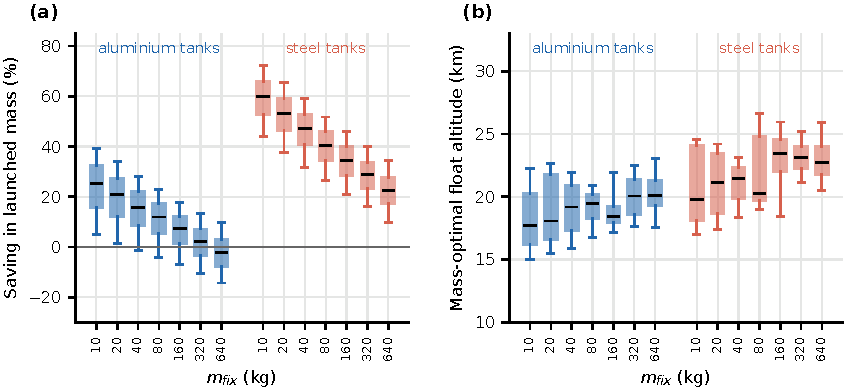
\includegraphics[width=\textwidth]{figures/fig_saving.pdf}
\caption{Monte Carlo over the rockoon-only penalties (\R{mcsN} samples per family; boxes span the quartiles and whiskers the 5th--95th percentiles). (a) Saving in launched mass against a ground-launched vehicle designed for ground launch. (b) Mass-optimal float altitude.}
\label{fig:saving}
\end{figure}

\begin{table}[!htb]
\centering
\caption{Lift-off mass (kg) of ground-launched vehicles that reach 100\,km and of the rockoon at its optimum with the central penalties (10\,kg\,m$^{-2}$ nozzle wall, 20\% gondola, $k=0.1$). ``Same design'': the balloon vehicle's proportions, thrust and nozzle rule; ``one stage'' and ``two stages'': designed for ground launch. The saving is against the lighter ground-launched option; $P$ is the probability of a saving in the Monte Carlo, against the single-stage option.}
\label{tab:comparators}
\small
\begin{tabular}{ccccccccc}
\toprule
Tanks & $m_{\mathrm{fix}}$ & \multicolumn{3}{c}{Ground launch} & \multicolumn{2}{c}{Rockoon} & Saving & $P$ \\
 & (kg) & same design & one stage & two stages & launched & $z^{*}$ (km) & (\%) & (\%) \\
\midrule
\tabin{tab_comparators.tex}
\bottomrule
\end{tabular}
\end{table}

\section{Where the apogee gain comes from}
\label{sec:gain}

The companion question, why a balloon launch reaches higher, is treated in full in the supplementary file. Its results are summarised here because they explain the shape of the curves used above.

Ignited at rest at 30\,km, the baseline vehicle reaches \R{balAp}\,km; launched from the ground with the nozzle that the selection rule gives there, it reaches \R{gndAp}\,km. A balloon changes three things at once: the rocket starts higher (head start), it flies through thinner air (drag), and its nozzle can have a larger area ratio and sees a lower back-pressure (nozzle). The trajectory code can switch each of the three between the ground and the float altitude, which gives eight runs. The effects are not additive, so we attribute the gain by averaging each contribution over the six orders of switching, which is the Shapley value of cooperative game theory \cite{shapley1953}. Drag accounts for \R{decFDrag}\% of the \R{gainKm}\,km gain, the nozzle for \R{decFNozzle}\% and the head start for \R{decFHead}\% (Fig.~\ref{fig:decomp}). The average hides a dependence on the order (the drag contribution is \R{ordDragLo}--\R{ordDragHi}\%), and the split depends on the drag calibration of Sec.~\ref{sec:validation}: the drag share is \R{cdTwoFDrag}\% if the drag is twice that assumed. In burnout velocity the split is \R{dvbFDrag}/\R{dvbFNozzle}/\R{dvbFHead}\%. The nozzle term is large because a pressure-fed engine has a low chamber pressure, so that a nozzle that does not separate at sea level is limited to an area ratio of about \R{gndEps}, while at 30\,km the limit is set by the body diameter ($\varepsilon=\R{balEps}$). When each vehicle is designed for its own launch the apogee ratio falls from \R{gainRatio} to \R{optRatio}. Most of the benefit is collected low down: over the first 10\,km the apogee rises by \R{gndFirstTen}\,km for each kilometre of ignition altitude, but between 20 and 30\,km by only \R{altGainLow}\,km, while the balloon volume grows by a factor of \R{altVolRatioLow}. This is why the saving per kilometre in Eq.~(\ref{eq:rule}) decays over a length $L$ of about 10\,km.

\begin{figure}[!htb]
\centering
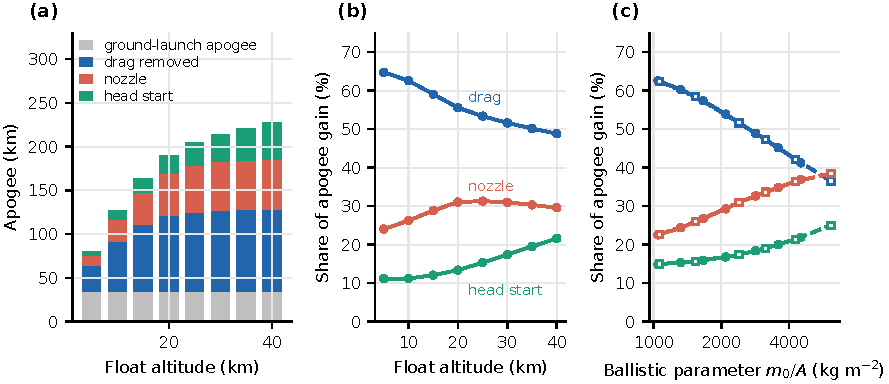
\includegraphics[width=\textwidth]{figures/fig_decomposition.pdf}
\caption{Decomposition of the apogee gain. (a) Baseline vehicle against float altitude: ground-launch apogee and the three contributions. (b) The same as shares of the gain. (c) Shares at a float altitude of 30\,km against the ballistic parameter. Colours as in (b). Filled symbols: gross mass varied from 25 to 2000\,kg at constant proportions. Open symbols: diameter of the 301\,kg vehicle varied from 0.25 to 0.60\,m.}
\label{fig:decomp}
\end{figure}

Three further results bear on the design of a rockoon. First, the drag loss of a ground launch is governed by one known group, the ratio of the air column above the vehicle to its ballistic coefficient, $\Pi_D=C_DA\,p(z_0)/(m_0g_0)$ \cite{allen1958}. Over \R{ensN} random vehicles with four engine types it explains \R{fitLdOne} of the variance of the ground-launch drag loss, although not the shares of the gain (\R{fitSdOne} for the drag share). Second, variance-based sensitivity indices \cite{jansen1999,saltelli2010} show that the drag coefficient, which carries \R{sobCdZero} of the apogee variance of a ground launch, stops mattering once $\Pi_D(z_0)$ falls below about 0.2, which happens at \R{h3ZLo}--\R{h3ZHi}\,km for four vehicles of very different size. Above that altitude the apogee uncertainty is set by the dry mass and the engine efficiency, which can be measured on the ground. Third, a rocket fired from a balloon must hold its attitude through the first seconds of the burn. With the thrust direction held, a tilt of 10$^{\circ}$ costs \R{tiltFixedLossTen}\% of the apogee, but a gravity turn from rest at 30\,km would cost \R{tiltTurnLossTen}\%, which is the problem that the suspended-launcher experiments address \cite{shoyama2021,shoyama2026}.

\section{Discussion}

\subsection{Answers to the questions}

\emph{Which float altitude.} When the balloon is counted, the launched mass is smallest at \R{zsLo}--\R{zsHi}\,km with a film of fixed areal density and at \R{grFitZLo}--\R{grFitZHi}\,km with an envelope law fitted to published balloons, for vehicles differing by a factor of fifty in mass. The minimum is flat: with the film law anything between \R{zsBandLo} and \R{zsBandHi}\,km is within 5\% of the best. The design rule does not depend on the propellant: float near 20\,km, not as high as possible. The optimum moved by at most a few kilometres under every penalty, comparator and cost weighting we tried, and stayed within \R{mcsZLo}--\R{mcsZHi}\,km over the Monte Carlo.

\emph{Why, and what moves it.} Most of the drag and nozzle benefit is collected in the first two or three scale heights of the atmosphere, while the balloon volume grows six- to ninefold for each further 10\,km. Equation~(\ref{eq:general}) makes this exact for any envelope law: at the optimum the envelope is the fraction $1/(\alpha\Lambda/H_\rho-\beta)$ of the suspended mass. Because the saving decays and the envelope grows exponentially with altitude, every input moves the optimum only through a logarithm multiplied by $L_{\mathrm{eff}}$, which is 3--7\,km. The kind of balloon decides the rest. An envelope that grows more slowly than its load puts the optimum higher for larger vehicles, and one that grows faster puts it lower. A cluster of identical latex balloons has a shorter $L_{\mathrm{eff}}$ and an optimum that does not depend on the gondola. A price on the balloon system can lower the optimum by at most \R{grInfFallHi}\,km, and a cheap envelope raises it towards the balloon's ceiling, which is where Okninski \emph{et al.} \cite{okninski2016} found it. The altitudes that programmes have stated lie mostly near 20\,km, and the exceptions include those for which the rocket is dear beside the balloon.

\emph{Whether a rockoon saves mass.} Only if the rocket's dry structure is heavy. Against ground-launched vehicles designed for ground launch, including two-stage ones, and with the hardware that only a rockoon needs, a pressure-fed rocket with steel tanks saves \R{liqBestSaveSsLo}--\R{liqBestSaveSsHi}\% of the launched mass, and does so in practically every Monte Carlo sample. With aluminium tanks the saving is \R{liqBestSaveAlLo} to \R{liqBestSaveAlHi}\%, and with the tank mass of a flown pressure-fed stage it is \R{rdAbSaveLo} to \R{rdAbSaveHi}\%. With solid motors it is \R{solSaveLo} to \R{solSaveHi}\% for a generic motor of high mass fraction and \R{rdSolSlSaveLo}--\R{rdSolSlSaveHi}\% with the inert mass of a flown booster. A rockoon is therefore most attractive where a light ground-launched rocket cannot be built.

\emph{Where the gain comes from.} For a pressure-fed vehicle of a few hundred kilograms ignited at 30\,km, about half of the apogee gain is drag that is no longer paid, about three tenths is the nozzle, and the rest is the head start. Above the altitude at which $\Pi_D(z_0)$ falls to about 0.2, which is 11--20\,km for the vehicles tested, the drag coefficient no longer contributes to the apogee uncertainty, so a balloon launch removes the quantity that is hardest to predict without wind-tunnel or flight data.

\subsection{Limitations}

The trajectory in the main results is vertical and one-dimensional; a planar model is used for the Super Loki check and for the tilt study of the supplementary file. Wind, balloon swing and attitude dynamics are not modelled. A rocket hanging under a balloon has essentially no dynamic pressure at ignition, so fins cannot stabilise it, and it swings; Shoyama \emph{et al.} \cite{shoyama2026} report that elevation oscillation of a suspended launcher is still an open problem, and we represent the launcher and attitude-control hardware only by a gondola mass. The model also ignores the balloon as an obstacle. A rocket fired vertically from beneath a balloon has to pass through it or beside it; for a hydrogen balloon and a hypergolic engine this would need a separate safety analysis.

The baseline drag curve is assumed, though it lies close to a curve computed for a definite geometry. It does not grow with fineness; Sec.~\ref{sec:saving} corrects for the wetted area of a slender body but not for the structure it needs. The curve reproduces six of the eight Deacon ground rounds to within about 3\%, but those flights cover only the first three seconds and a different body; with the Super Loki report's own drag tables the model over-predicts that rocket's apogee by about 6\%, and it over-predicts four Aerobee flights by about \R{abFltMean}\%. The rockoon comparison needs one fitted mass per group of flights; the only independent mass we found comes from a secondary compilation and, with it, the model over-predicts the flights. We have not been able to consult the original accounts \cite{vanallen1954,vanallen1959}, which may give the payloads. The thermochemistry agrees with NASA CEA, and the efficiency of 0.92 is close to the \R{abEtaVac} of the Aerobee engine, but no engine burning our propellants has been compared with flight. The item masses of the Aerobee come from a secondary compilation. Tank and bottle masses are those of ideal thin-walled spheres with one correction factor, helium is treated as an ideal gas, and no knock-down is applied for welded aluminium; the Aerobee value shows that flown tanks can be lighter than our aluminium estimate. The fitted envelope law rests on eleven balloons, none carrying a load as heavy for its size as a rockoon, and the latex law rests on catalogue burst diameters, not on tests with heavy loads. The balloon model neglects superheat, ascent dynamics and the natural shape of the envelope, and the condition of Sec.~\ref{sec:analytic} is exact for the model, not for a real balloon. Except in Sec.~\ref{sec:saving}, the ground- and balloon-launched vehicles share one thrust-to-weight ratio and one body. The two-stage and solid comparators use assumed booster fixed masses and a generic solid motor. The table of programme altitudes rests partly on statements in the press. The thermal check of Sec.~\ref{sec:optimum} is a conduction estimate only. We have not attempted a structural or priced cost analysis.

\section{Conclusions}

\begin{enumerate}
\item The float altitude that minimises the launched mass for a 100\,km apogee is \R{zsLo}--\R{zsHi}\,km over a fifty-fold range of vehicle mass with a film of fixed areal density, and \R{grFitZLo}--\R{grFitZHi}\,km with an envelope law fitted to \R{envN} published balloons. Over a Monte Carlo of the rockoon-only penalties and the envelope law it stays within \R{mcsZLo}--\R{mcsZHi}\,km.
\item For any envelope law $m_e=E(V,m_s)$ the optimum satisfies Eq.~(\ref{eq:general}) exactly. For the launched mass the envelope is then the fraction $1/(\alpha\Lambda/H_\rho-\beta)$ of the suspended mass; for a film of fixed areal density it weighs $\tfrac32H_\rho$ times the suspended mass saved per kilometre of altitude. The optimum depends on every input only through a logarithm multiplied by $L_{\mathrm{eff}}=(1/L+\alpha_2/H_\rho)^{-1}$, 3--7\,km, and not on the ground-launched comparator. One step of Eq.~(\ref{eq:zstar}) from a trial design at 20\,km finds it to within \R{grStepOne}\,km.
\item The kind of balloon decides how the optimum moves. It rises with vehicle size when the envelope mass grows more slowly than the load ($\alpha+\beta<1$, the film law, $\R{grAreaSlope}$\,km per decade of mass) and falls when it grows faster (the fitted law, $\R{grFitSlope}$\,km per decade). For clusters of latex balloons it is \R{grCluZLo}--\R{grCluZHi}\,km. A price on the balloon system lowers it by at most \R{grInfFallLo}--\R{grInfFallHi}\,km, and a cheap envelope raises it towards the balloon's ceiling, which reconciles this result with the high altitudes found best in a cost study of latex clusters.
\item The saving is not robust. Against ground-launched vehicles designed for ground launch, including two-stage ones, and with the central rockoon penalties, it is \R{liqBestSaveSsLo}--\R{liqBestSaveSsHi}\% for pressure-fed vehicles with steel tanks (probability of a saving at least \R{mcsSsPLo}\%), \R{liqBestSaveAlLo} to \R{liqBestSaveAlHi}\% with aluminium tanks (probability \R{mcsAlPLo}--\R{mcsAlPHi}\%), \R{rdAbSaveLo} to \R{rdAbSaveHi}\% with the tank mass of the Aerobee~150A, and \R{solSaveLo} to \R{solSaveHi}\% with a generic solid motor (\R{rdSolSlSaveLo}--\R{rdSolSlSaveHi}\% with the inert mass of a flown booster). It is decided by how heavy the rocket's dry structure is.
\item For a 301\,kg pressure-fed UDMH/N$_2$O$_4$ vehicle, ignition at 30\,km raises the apogee from \R{gndAp} to \R{balAp}\,km: \R{decFDrag}\% of the gain is drag, \R{decFNozzle}\% nozzle and \R{decFHead}\% head start. The ballistic drag parameter $\Pi_D$ collapses the drag loss of a ground launch (\R{fitLdOne} of the variance over \R{ensN} vehicles) but not the shares of the gain, and the drag coefficient stops contributing to the apogee uncertainty once $\Pi_D(z_0)$ falls to about 0.2.
\item The model reproduces six of eight NACA Deacon ground firings to within \R{deaErrMaxAbs}\% in maximum velocity and the nominal performance of the pressure-fed Aerobee~150 to within \R{abNomMax}\% in peak altitude; it over-predicts the Super Loki Dart apogee by about 6\% and four Aerobee flights by \R{abFltLo}--\R{abFltHi}\%, and reproduces the apogees of nine Deacon rockoon flights of 1952--53 to \R{rkAllRms}\% r.m.s. with one fitted mass per group. The delivered specific impulse of the Aerobee engine is \R{abEtaVac} of the ideal value by our method, against the 0.92 assumed. The thermochemistry agrees with NASA CEA to \R{ceaMaxDiff}\% and the trajectories with RocketPy to \R{rpMaxDiff}\%.
\end{enumerate}

\section*{Acknowledgements}

We thank the principal of CHIREC International School, to whom the original proposal was presented.

\section*{Declaration of generative AI use}

The authors used Claude (Anthropic), a generative AI model, in preparing this work: to review the authors' October 2026 draft, to search for and summarise related literature, to propose and compare candidate research questions and hypotheses, to write and run the analysis code, to produce the figures, and to draft the manuscript text. The 2022 proposal and the decision to revisit it are the authors' own. The authors reviewed the text, code, results and references and take full responsibility for the content of this paper.

\section*{Code and data availability}

\sloppy The scripts and the supplementary file are included with this submission as ancillary files, and are also at \url{https://github.com/FOUNDERACCRETION/rockoon-gain}. \texttt{rockoon\_model.py} holds the models; \texttt{similarity.py}, \texttt{extra\_tests.py}, \texttt{revision\_tests.py} and \texttt{realdata\_tests.py} run the ensemble, optimum, Sobol, design-search, two-stage, Monte Carlo and published-data calculations; \texttt{general\_rule.py} solves the envelope rule for each envelope law; \texttt{cea\_check.py}, \texttt{rocketpy\_check.py} and \texttt{aerobee\_check.py} run the checks against NASA CEA, RocketPy and the Aerobee~150; \texttt{run\_analysis.py}, \texttt{revision\_analysis.py} and \texttt{realdata\_analysis.py} compute every number; and \texttt{make\_tables.py}, \texttt{make\_figures.py} and \texttt{check\_paper.py} write the tables and figures and check the manuscript. They require Python 3.10 or later with NumPy, SciPy, Matplotlib, Cantera 3.2.0, \texttt{cea} 3.3.4 and RocketPy 1.13.0. Every number in the text that is computed is read from \texttt{results.tex}, which \texttt{run\_analysis.py} writes, and a single script, \texttt{run\_all.sh}, regenerates everything. The file \texttt{test\_model.py} contains checks of the model against values that can be worked out by hand, and \texttt{validate.py} runs every check in the paper.

\appendix

\section{Supplementary tables}
\label{app:tables}

\begin{table}[!htbp]
\centering
\caption{Deacon ground firings \cite{watson1949}: reported gross mass, total impulse and maximum velocity, and the maximum velocity computed with a drag scale factor of one.}
\label{tab:deacon}
\small
\begin{tabular}{cccccc}
\toprule
Round & Gross mass & Impulse & Measured $v_{\max}$ & Computed $v_{\max}$ & Difference \\
 & (kg) & (kN\,s) & (m\,s$^{-1}$) & (m\,s$^{-1}$) & (\%) \\
\midrule
\tabin{tab_deacon.tex}
\bottomrule
\end{tabular}
\end{table}

\begin{table}[!htbp]
\centering
\caption{Deacon rockoon firings \cite{smith1954}: firing altitude and zenith from the data sheets, and the apogee computed with one fitted gross mass per group (\R{rkSuiMass}\,kg for the Iowa flights, \R{rkNrlMass}\,kg for the NRL flights).}
\label{tab:rockoons}
\small
\begin{tabular}{lcccc}
\toprule
Flight & Firing altitude (km) & Zenith (km) & Computed (km) & Difference (\%) \\
\midrule
\tabin{tab_rockoons.tex}
\bottomrule
\end{tabular}
\end{table}

\begin{table}[!htbp]
\centering
\caption{Aerobee~150: nominal performance stated in the NASA compendia for net payloads of 150\,lb \cite{busse1966} and 250\,lb \cite{busse1967}, and four flights from White Sands in 1964 with stated net payload weights \cite{busse1967}, against the model flown vertically with the published thrust, flow rate and masses and a drag scale factor of one.}
\label{tab:aerobee}
\footnotesize
\begin{tabular}{@{}lcccccccc@{}}
\toprule
Case & Payload & Launch & \multicolumn{3}{c}{Peak altitude (km)} & \multicolumn{3}{c}{Burnout velocity (m\,s$^{-1}$)} \\
 & (kg) & elev. (m) & published & computed & (\%) & published & computed & (\%) \\
\midrule
\tabin{tab_aerobee.tex}
\bottomrule
\end{tabular}
\end{table}

\begin{table}[!htbp]
\centering
\caption{Vehicles that reach 100\,km with $m_{\mathrm{fix}}=80$\,kg. Balloon values are for the aluminium vehicle.}
\label{tab:closure}
\small
\begin{tabular}{ccccccc}
\toprule
Ignition & Propellant & \multicolumn{2}{c}{Gross mass (kg)} & \multicolumn{3}{c}{Balloon (Al vehicle)} \\
altitude (km) & (kg, Al) & Al tanks & steel tanks & volume (m$^3$) & envelope (kg) & H$_2$ (kg) \\
\midrule
\tabin{tab_closure.tex}
\bottomrule
\end{tabular}
\end{table}

\begin{table}[!htbp]
\centering
\caption{The envelope rule for the film law (Sec.~\ref{sec:analytic}) and the fourteen families: decay length $L$ of the rocket-mass saving, density scale height $H_\rho$ and $L_{\mathrm{eff}}$ of Eq.~(\ref{eq:zstar}); optimum of the full model and from Eq.~(\ref{eq:rule}); and the two sides of Eq.~(\ref{eq:rule}) at the optimum of the full model. The right side uses the slope of the fitted rocket curve rather than that of the closed vehicles, which is why the two sides differ by up to about 15\%.}
\label{tab:analytic}
\small
\begin{tabular}{ccccccccc}
\toprule
Tanks & $m_{\mathrm{fix}}$ & $L$ & $H_\rho$ & $L_{\mathrm{eff}}$ & $z^{*}$, model & $z^{*}$, Eq.~(\ref{eq:rule}) & $m_e$ & $\tfrac32H_\rho|dm_s/dz|$ \\
 & (kg) & (km) & (km) & (km) & (km) & (km) & (kg) & (kg) \\
\midrule
\tabin{tab_analytic.tex}
\bottomrule
\end{tabular}
\end{table}

\section{Safety note}
\label{app:hazards}

UDMH is a possible human carcinogen (IARC Group 2B) with a NIOSH exposure ceiling of 0.06\,ppm, and nitrogen dioxide, in equilibrium with N$_2$O$_4$, has a short-term limit of 1\,ppm \cite{iarc,nioshudmh,nioshno2}; nothing in this paper suggests these propellants are suitable for school or amateur use.

\begin{thebibliography}{99}

\bibitem{ludwig2004} G.\,H. Ludwig, \emph{James Alfred Van Allen: From High School to the Beginning of the Space Era, A Biographical Sketch} (University of Iowa, Iowa City, 9 October 2004), pp.~7--8, \url{https://space.physics.uiowa.edu/plasma-wave/van90/VanAllenBio_LudwigOct2004.pdf}.

\bibitem{corliss1971} W.\,R. Corliss, \emph{NASA Sounding Rockets, 1958--1968: A Historical Summary}, NASA SP-4401 (National Aeronautics and Space Administration, Washington, DC, 1971).

\bibitem{vanallen1954} J.\,A. Van Allen and M.\,B. Gottlieb, ``The inexpensive attainment of high altitudes with balloon-launched rockets,'' in \emph{Rocket Exploration of the Upper Atmosphere}, edited by R.\,L.\,F. Boyd and M.\,J. Seaton (Pergamon Press, London, 1954), pp.~53--64.

\bibitem{vanallen1959} J.\,A. Van Allen, ``Balloon-launched rockets for high-altitude research,'' in \emph{Sounding Rockets}, edited by H.\,E. Newell, Jr. (McGraw-Hill, New York, 1959), Chap.~9, pp.~143--164.

\bibitem{okninski2016} A. Okninski, D. Sors Raurell, and A. Rodriguez Mitre, ``Feasibility of a low-cost sounding rockoon platform,'' Acta Astronaut. \textbf{127}, 335--344 (2016), doi:10.1016/j.actaastro.2016.06.010.

\bibitem{li2022} J. Li, K. Peng, W. Wang, Z. Wu, and W. Zhang, ``Optimization design of rockoons based on improved sequential approximation optimization,'' Proc. Inst. Mech. Eng. G: J. Aerosp. Eng. \textbf{236}, 140--153 (2022), doi:10.1177/09544100211008604.

\bibitem{jorda2012} R. Jorda-Siquier, ``Rockoon suitability for launching small satellites into LEO orbits,'' in \emph{63rd International Astronautical Congress}, paper IAC-12-D2.7.4 (Naples, 2012).

\bibitem{shoyama2022} T. Shoyama, Y. Wada, and T. Matsui, ``Conceptual study on low-melting-point thermoplastic fuel/nitrous oxide hybrid rockoon,'' J. Spacecr. Rockets \textbf{59}, 286--294 (2022), doi:10.2514/1.A35040.

\bibitem{shoyama2021} T. Shoyama, A. Banno, Y. Furuta, N. Kurata, D. Ode, Y. Wada, and T. Matsui, ``Air-launch experiment using suspended rail launcher for rockoon,'' Aerospace \textbf{8}, 289 (2021), doi:10.3390/aerospace8100289.

\bibitem{shoyama2026} T. Shoyama, Y. Wada, and S. Oda, ``Rockoon launch experiment with azimuth angle control,'' Aerospace \textbf{13}, 709 (2026), doi:10.3390/aerospace13080709.

\bibitem{bloostar2015} A. Schoenmaker \emph{et al.}, ``Bloostar: a balloon-assisted lightweight launcher to orbit microsatellites,'' in \emph{66th International Astronautical Congress}, paper IAC-15-D2.7.8 (Jerusalem, 2015).

\bibitem{jaxa2026} Japan Aerospace Exploration Agency, ``AstroX and JAXA begin joint business demonstration activities for a suspension-type attitude control device for stratospheric balloon applications,'' press release, 28 May 2026, \url{https://global.jaxa.jp/press/2026/05/20260528-1_e.html}.

\bibitem{tsien1951} H.\,S. Tsien and R.\,C. Evans, ``Optimum thrust programming for a sounding rocket,'' J. Am. Rocket Soc. \textbf{21}, 99--107 (1951), doi:10.2514/8.4372.

\bibitem{sarigul2005} N. Sarigul-Klijn, M. Sarigul-Klijn, and C. Noel, ``Air-launching Earth to orbit: effects of launch conditions and vehicle aerodynamics,'' J. Spacecr. Rockets \textbf{42}, 569--575 (2005), doi:10.2514/1.8634.

\bibitem{janhunen2018} P. Janhunen, P. Toivanen, and K. Ruosteenoja, ``Steam balloon concept for lifting rockets to launch altitude,'' Aeronaut. J. \textbf{123}, 600--616 (2019), doi:10.1017/aer.2019.10.

\bibitem{ussa1976} \emph{U.S. Standard Atmosphere, 1976}, NOAA-S/T 76-1562 (National Oceanic and Atmospheric Administration, National Aeronautics and Space Administration, and U.S. Air Force, Washington, DC, 1976).

\bibitem{yajima2009} N. Yajima, N. Izutsu, T. Imamura, and T. Abe, \emph{Scientific Ballooning: Technology and Applications of Exploration Balloons Floating in the Stratosphere and the Atmospheres of Other Planets} (Springer, New York, 2009), doi:10.1007/978-0-387-09727-5.

\bibitem{csbf} NASA Columbia Scientific Balloon Facility, ``Balloons,'' \url{https://csbf.nasa.gov/balloons.html} (accessed 18 November 2026).

\bibitem{nasaldb} National Aeronautics and Space Administration, ``Long duration balloon opportunities,'' Small Explorer Class Library (NASA, 2003), \url{https://explorers.larc.nasa.gov/PDF_FILES/LDB_SMEX_03_Rev4.pdf} (accessed 18 November 2026).

\bibitem{aerostar2005} Aerostar International, ``Small zero pressure balloons: performance curves and balloon weights,'' Rev. 17 February 2005, \url{https://cdn.ravenaerostar.com/legacy/aerospace/Aerostar_small_zero_pressure_performance_curves.pdf} (accessed 18 November 2026).

\bibitem{rainwater2004} E.\,L. Rainwater and M.\,S. Smith, ``Ultra high altitude balloons for medium-to-large payloads,'' Adv. Space Res. \textbf{33}, 1648 (2004), doi:10.1016/j.asr.2003.07.037.

\bibitem{gordon1994} S. Gordon and B.\,J. McBride, \emph{Computer Program for Calculation of Complex Chemical Equilibrium Compositions and Applications. I. Analysis}, NASA Reference Publication 1311 (NASA Lewis Research Center, Cleveland, OH, 1994).

\bibitem{cantera} D.\,G. Goodwin, H.\,K. Moffat, I. Schoegl, R.\,L. Speth, and B.\,W. Weber, \emph{Cantera: An Object-Oriented Software Toolkit for Chemical Kinetics, Thermodynamics, and Transport Processes}, version 3.2.0 (2025), \url{https://www.cantera.org}, doi:10.5281/zenodo.17620923.

\bibitem{mcbride2002} B.\,J. McBride, M.\,J. Zehe, and S. Gordon, \emph{NASA Glenn Coefficients for Calculating Thermodynamic Properties of Individual Species}, NASA/TP-2002-211556 (NASA Glenn Research Center, Cleveland, OH, 2002).

\bibitem{nist} P.\,J. Linstrom and W.\,G. Mallard, eds., \emph{NIST Chemistry WebBook}, NIST Standard Reference Database Number 69 (National Institute of Standards and Technology, Gaithersburg, MD), \url{https://webbook.nist.gov} (accessed 18 November 2026).

\bibitem{astronautix} M. Wade, ``N2O4/UDMH,'' in \emph{Encyclopedia Astronautica}, \url{http://www.astronautix.com/n/n2o4udmh.html} (accessed 18 November 2026).

\bibitem{cea2026} National Aeronautics and Space Administration, \emph{CEA: Chemical Equilibrium with Applications}, version 3.3.4, Python package, \url{https://nasa.github.io/cea} (accessed 18 November 2026).

\bibitem{scipy} P. Virtanen \emph{et al.}, ``SciPy 1.0: fundamental algorithms for scientific computing in Python,'' Nat. Methods \textbf{17}, 261--272 (2020).

\bibitem{niskanen2009} S. Niskanen, \emph{Development of an Open Source Model Rocket Simulation Software}, M.Sc. thesis (Helsinki University of Technology, 2009).

\bibitem{niskanen2013} S. Niskanen, \emph{OpenRocket Technical Documentation, for OpenRocket version 13.05} (10 May 2013), \url{https://openrocket.sourceforge.net/techdoc.pdf}.

\bibitem{traveler} A. Aitoumeziane, P. Eusebio, C. Hayes, V. Ramachandran, J. Smith, J. Sridharan, L. St.~Regis, M. Stephenson, N. Tewksbury, M. Tran, and H. Yang, ``Traveler IV apogee analysis,'' white paper (USC Rocket Propulsion Laboratory, Los Angeles, May 2019), \url{http://www.uscrpl.com/s/Traveler-IV-Whitepaper}.

\bibitem{bollermann1968} B. Bollermann and R.\,L. Walker, \emph{Super Loki Dart Meteorological Rocket System}, NASA CR-61238 (Space Data Corporation, Phoenix, AZ, 30 June 1968), \url{https://ntrs.nasa.gov/citations/19680026183}.

\bibitem{asm} ASM International, \emph{ASM Handbook, Vol.~2: Properties and Selection: Nonferrous Alloys and Special-Purpose Materials} (ASM International, Materials Park, OH, 1990).

\bibitem{astm} ASTM International, \emph{ASTM A240/A240M-20a: Standard Specification for Chromium and Chromium-Nickel Stainless Steel Plate, Sheet, and Strip for Pressure Vessels and for General Applications} (ASTM International, West Conshohocken, PA, 2020).

\bibitem{busse1966} J.\,R. Busse and M.\,T. Leffler, \emph{A Compendium of Aerobee Sounding Rocket Launchings From 1959 Through 1963}, NASA TR R-226 (National Aeronautics and Space Administration, Washington, DC, 1966), \url{https://ntrs.nasa.gov/citations/19660005621}.

\bibitem{openaerospace} Open Aerospace, ``Aerobee 150,'' \url{https://open-aerospace.github.io/Aerobee-150} (accessed 19 November 2026).

\bibitem{watson1949} R.\,S. Watson, \emph{Flight Investigation of 6.25-Inch-Diameter Deacon Rocket and 10-Inch-Scale Model Rocket}, NACA Research Memorandum RM L8H26 (Langley Aeronautical Laboratory, Langley Air Force Base, VA, 25 March 1949), \url{https://ntrs.nasa.gov/citations/20050019279}.

\bibitem{smith1954} C.\,P. Smith, Jr., \emph{Summary of Upper Atmosphere Rocket Research Firings}, Upper Atmosphere Research Report No.~XXI, NRL Report 4276 (Naval Research Laboratory, Washington, DC, February 1954), with supplementary pages by E.\,C. Pressly (February 1958), \url{https://apps.dtic.mil/sti/tr/pdf/ADB957191.pdf}.

\bibitem{astronautixdeacon} M. Wade, ``Deacon Rockoon,'' in \emph{Encyclopedia Astronautica}, \url{http://www.astronautix.com/d/deaconrockoon.html} (accessed 18 November 2026).

\bibitem{busse1967} J.\,R. Busse, M.\,T. Leffler, G.\,E. Kraft, and P.\,S. Bushnell, Jr., \emph{A Compendium of NASA Aerobee Sounding Rocket Launchings for 1964} (National Aeronautics and Space Administration, Washington, DC, July 1967), \url{https://ntrs.nasa.gov/citations/19670025553}.

\bibitem{rocketpy2021} G.\,H. Ceotto, R.\,N. Schmitt, G.\,F. Alves, L.\,A. Pezente, and B.\,S. Carmo, ``RocketPy: six degree-of-freedom rocket trajectory simulator,'' J. Aerosp. Eng. \textbf{34}(6) (2021), doi:10.1061/(ASCE)AS.1943-5525.0001331.

\bibitem{kaymont} Rocketman Enterprises, ``High altitude weather balloons (HAB),'' specifications of the Kaymont (Totex) HAB series, \url{https://the-rocketman.com/products/high-altitude-weather-balloons-hab} (accessed 19 November 2026).

\bibitem{farside} StratoCat, ``Far Side project, flight no.~6, 22 October 1957,'' \url{https://stratocat.com.ar/fichas-e/1957/ENW-19571022.htm} (accessed 19 November 2026).

\bibitem{arca2010} N. Atkinson, ``Moon balloon has mostly successful test flight,'' Universe Today, 5 October 2010, \url{https://universetoday.com/74983/moon-balloon-has-mostly-successful-test-flight}.

\bibitem{eoportal} eoPortal, ``Zero 2 Infinity,'' \url{https://eoportal.org/satellite-missions/zero-2-infinity} (accessed 19 November 2026).

\bibitem{purdue2018} Purdue University, ``\,`Rockoons' may soon make launching satellites into space more accessible,'' news release, 4 April 2018, \url{https://www.purdue.edu/newsroom/releases/2018/Q2/rockoons-may-soon-make-launching-satellites-into-space-more-accessible.html}.

\bibitem{ansys2021} Ansys, ``Hitching a balloon ride to space,'' Ansys Blog, 14 December 2021, \url{https://www.ansys.com/blog/hitching-a-balloon-ride-to-space}.

\bibitem{b2space} B2Space, ``Satellite launch,'' \url{https://b2-space.com/satellite-launch/} (accessed 19 November 2026).

\bibitem{parsonson2025} A. Parsonson, ``B2Space tests balloon-based launch system,'' European Spaceflight, 22 November 2025, \url{https://europeanspaceflight.com/?p=5587}.

\bibitem{jiji2024} Jiji Press, ``Fukushima startup aiming to launch rocket from flying balloon,'' Nippon.com, 22 December 2024, \url{https://www.nippon.com/en/news/yjj2024122100355/}.

\bibitem{sutton2017} G.\,P. Sutton and O. Biblarz, \emph{Rocket Propulsion Elements}, 9th ed. (Wiley, Hoboken, NJ, 2017).

\bibitem{shapley1953} L.\,S. Shapley, ``A value for $n$-person games,'' in \emph{Contributions to the Theory of Games II}, edited by H.\,W. Kuhn and A.\,W. Tucker, Annals of Mathematics Studies \textbf{28} (Princeton University Press, Princeton, NJ, 1953), pp.~307--317.

\bibitem{allen1958} H.\,J. Allen and A.\,J. Eggers, Jr., \emph{A Study of the Motion and Aerodynamic Heating of Ballistic Missiles Entering the Earth's Atmosphere at High Supersonic Speeds}, NACA Report 1381 (National Advisory Committee for Aeronautics, Washington, DC, 1958).

\bibitem{jansen1999} M.\,J.\,W. Jansen, ``Analysis of variance designs for model output,'' Comput. Phys. Commun. \textbf{117}, 35--43 (1999), doi:10.1016/S0010-4655(98)00154-4.

\bibitem{saltelli2010} A. Saltelli, P. Annoni, I. Azzini, F. Campolongo, M. Ratto, and S. Tarantola, ``Variance based sensitivity analysis of model output. Design and estimator for the total sensitivity index,'' Comput. Phys. Commun. \textbf{181}, 259--270 (2010).

\bibitem{iarc} International Agency for Research on Cancer, \emph{IARC Monographs on the Evaluation of Carcinogenic Risks to Humans, Vol.~71: Re-evaluation of Some Organic Chemicals, Hydrazine and Hydrogen Peroxide} (IARC, Lyon, 1999).

\bibitem{nioshudmh} National Institute for Occupational Safety and Health, ``NIOSH Pocket Guide to Chemical Hazards: 1,1-Dimethylhydrazine,'' \url{https://www.cdc.gov/niosh/npg/npgd0227.html} (accessed 18 November 2026).

\bibitem{nioshno2} National Institute for Occupational Safety and Health, ``NIOSH Pocket Guide to Chemical Hazards: Nitrogen dioxide,'' \url{https://www.cdc.gov/niosh/npg/npgd0454.html} (accessed 18 November 2026).

\end{thebibliography}

\end{document}
